\documentclass[supercite]{Experimental_Report}

%\title{基于高级语言源程序格式处理工具}
\title{~~~~~~基于高级语言源程序格式处理工具~~~~~~}
\author{崔昊阳}
\school{计算机科学与技术学院}
\classnum{CS2104}
\stunum{U202115415}
\instructor{袁凌}
\date{2022年8月30日}

\usepackage{algorithm, multirow}
\usepackage{algpseudocode}
\usepackage{amsmath}
\usepackage{amsthm}
\usepackage{framed}
\usepackage{mathtools}
\usepackage{subcaption}
\usepackage{xltxtra} %提供了针对XeTeX的改进并且加入了XeTeX的LOGO, 自动调用xunicode宏包(提供Unicode字符宏)
\usepackage{bm}
\usepackage{tikz}
\usepackage{tikzscale}
\usepackage{pgfplots}
%\usepackage{enumerate}
\usepackage{caption}
% \usepackage[dvipsnames]{xcolor}  % 更全的色系
\usepackage{listings}  % 排代码用的宏包
\lstset{
    language = C,
    backgroundcolor = \color{white},    % 背景色
    basicstyle = \small\ttfamily,           % 基本样式 + 小号字体
    rulesepcolor= \color{gray},             % 代码块边框颜色
    breaklines = true,                  % 代码过长则换行
    numbers = left,                     % 行号在左侧显示
    numberstyle = \small,               % 行号字体
    keywordstyle = \color{blue}\bfseries,      % 关键字颜色
    commentstyle =\color{green},        % 注释颜色
    stringstyle = \color{red},          % 字符串颜色
    frame = shadowbox,                  % 用(带影子效果)方框框住代码块
    showspaces = false,                 % 不显示空格
    columns = fixed,                    % 字间距固定
    %escapeinside={<@}{@>}              % 特殊自定分隔符:<@可以自己加颜色@>
    morekeywords = {as},                % 自加新的关键字(必须前后都是空格)
    deletendkeywords = {compile}        % 删除内定关键字;删除错误标记的关键字用deletekeywords删!
}


\pgfplotsset{compat=1.16}

\newcommand{\cfig}[3]{
  \begin{figure}[htb]
    \centering
    \includegraphics[width=#2\textwidth]{images/#1.tikz}
    \caption{#3}
    \label{fig:#1}
  \end{figure}
}

\newcommand{\sfig}[3]{
  \begin{subfigure}[b]{#2\textwidth}
    \includegraphics[width=\textwidth]{images/#1.tikz}
    \caption{#3}
    \label{fig:#1}
  \end{subfigure}
}

\newcommand{\xfig}[3]{
  \begin{figure}[htb]
    \centering
    #3
    \caption{#2}
    \label{fig:#1}
  \end{figure}
}

\newcommand{\rfig}[1]{\autoref{fig:#1}}
\newcommand{\ralg}[1]{\autoref{alg:#1}}
\newcommand{\rthm}[1]{\autoref{thm:#1}}
\newcommand{\rlem}[1]{\autoref{lem:#1}}
\newcommand{\reqn}[1]{\autoref{eqn:#1}}
\newcommand{\rtbl}[1]{\autoref{tbl:#1}}

\algnewcommand\Null{\textsc{null }}
\algnewcommand\algorithmicinput{\textbf{Input:}}
\algnewcommand\Input{\item[\algorithmicinput]}
\algnewcommand\algorithmicoutput{\textbf{Output:}}
\algnewcommand\Output{\item[\algorithmicoutput]}
\algnewcommand\algorithmicbreak{\textbf{break}}
\algnewcommand\Break{\algorithmicbreak}
\algnewcommand\algorithmiccontinue{\textbf{continue}}
\algnewcommand\Continue{\algorithmiccontinue}
\algnewcommand{\LeftCom}[1]{\State $\triangleright$ #1}

\newtheorem{thm}{定理}[section]
\newtheorem{lem}{引理}[section]

\colorlet{shadecolor}{black!15}

\theoremstyle{definition}
\newtheorem{alg}{算法}[section]

\def\thmautorefname~#1\null{定理~#1~\null}
\def\lemautorefname~#1\null{引理~#1~\null}
\def\algautorefname~#1\null{算法~#1~\null}

\begin{document}

\maketitle

\clearpage

\pagenumbering{Roman}

\tableofcontents[level=2]

\clearpage

\pagenumbering{arabic}

\section{问题描述}

在计算机科学中,抽象语法树(abstract syntax tree或者缩写为AST),
是将源代码的语法结构的用树的形式表示,树上的每个结点都表示源程序代码中的一种语法成分。
之所以说是“抽象”,是因为在抽象语法树中,忽略了源程序中语法成分的一些细节,突出了其主要语法特征。

抽象语法树(Abstract Syntax Tree ,AST)作为程序的一种中间表示形式,在程序分析等诸多领域有广泛的应用。
利用抽象语法树可以方便地实现多种源程序处理工具,比如源程序浏览器、智能编辑器、语言翻译器等。

在高级语言源程序格式处理工具的实现中,我们首先需要采用形式化的方式,使用巴克斯(BNF)范式定义高级语言的词法规则
(字符组成单词的规则)、语法规则(单词组成语句、程序等的规则)。再利用形式语言自动机的的原理,对源程序的文件进行词法分析,识别出所有单词;
使用编译技术中的递归下降语法分析法,分析源程序的语法结构,并生成抽象语法树,最后可由抽象语法树生成格式化的源程序。
\newpage
\section{程序的总体设计}

高级语言源程序格式处理工具由词法分析器(lexer)、语法分析器(parser)和AST生成工具构成。
它的文件结构如图所示。
\begin{figure}[htb]
	\begin{center}
		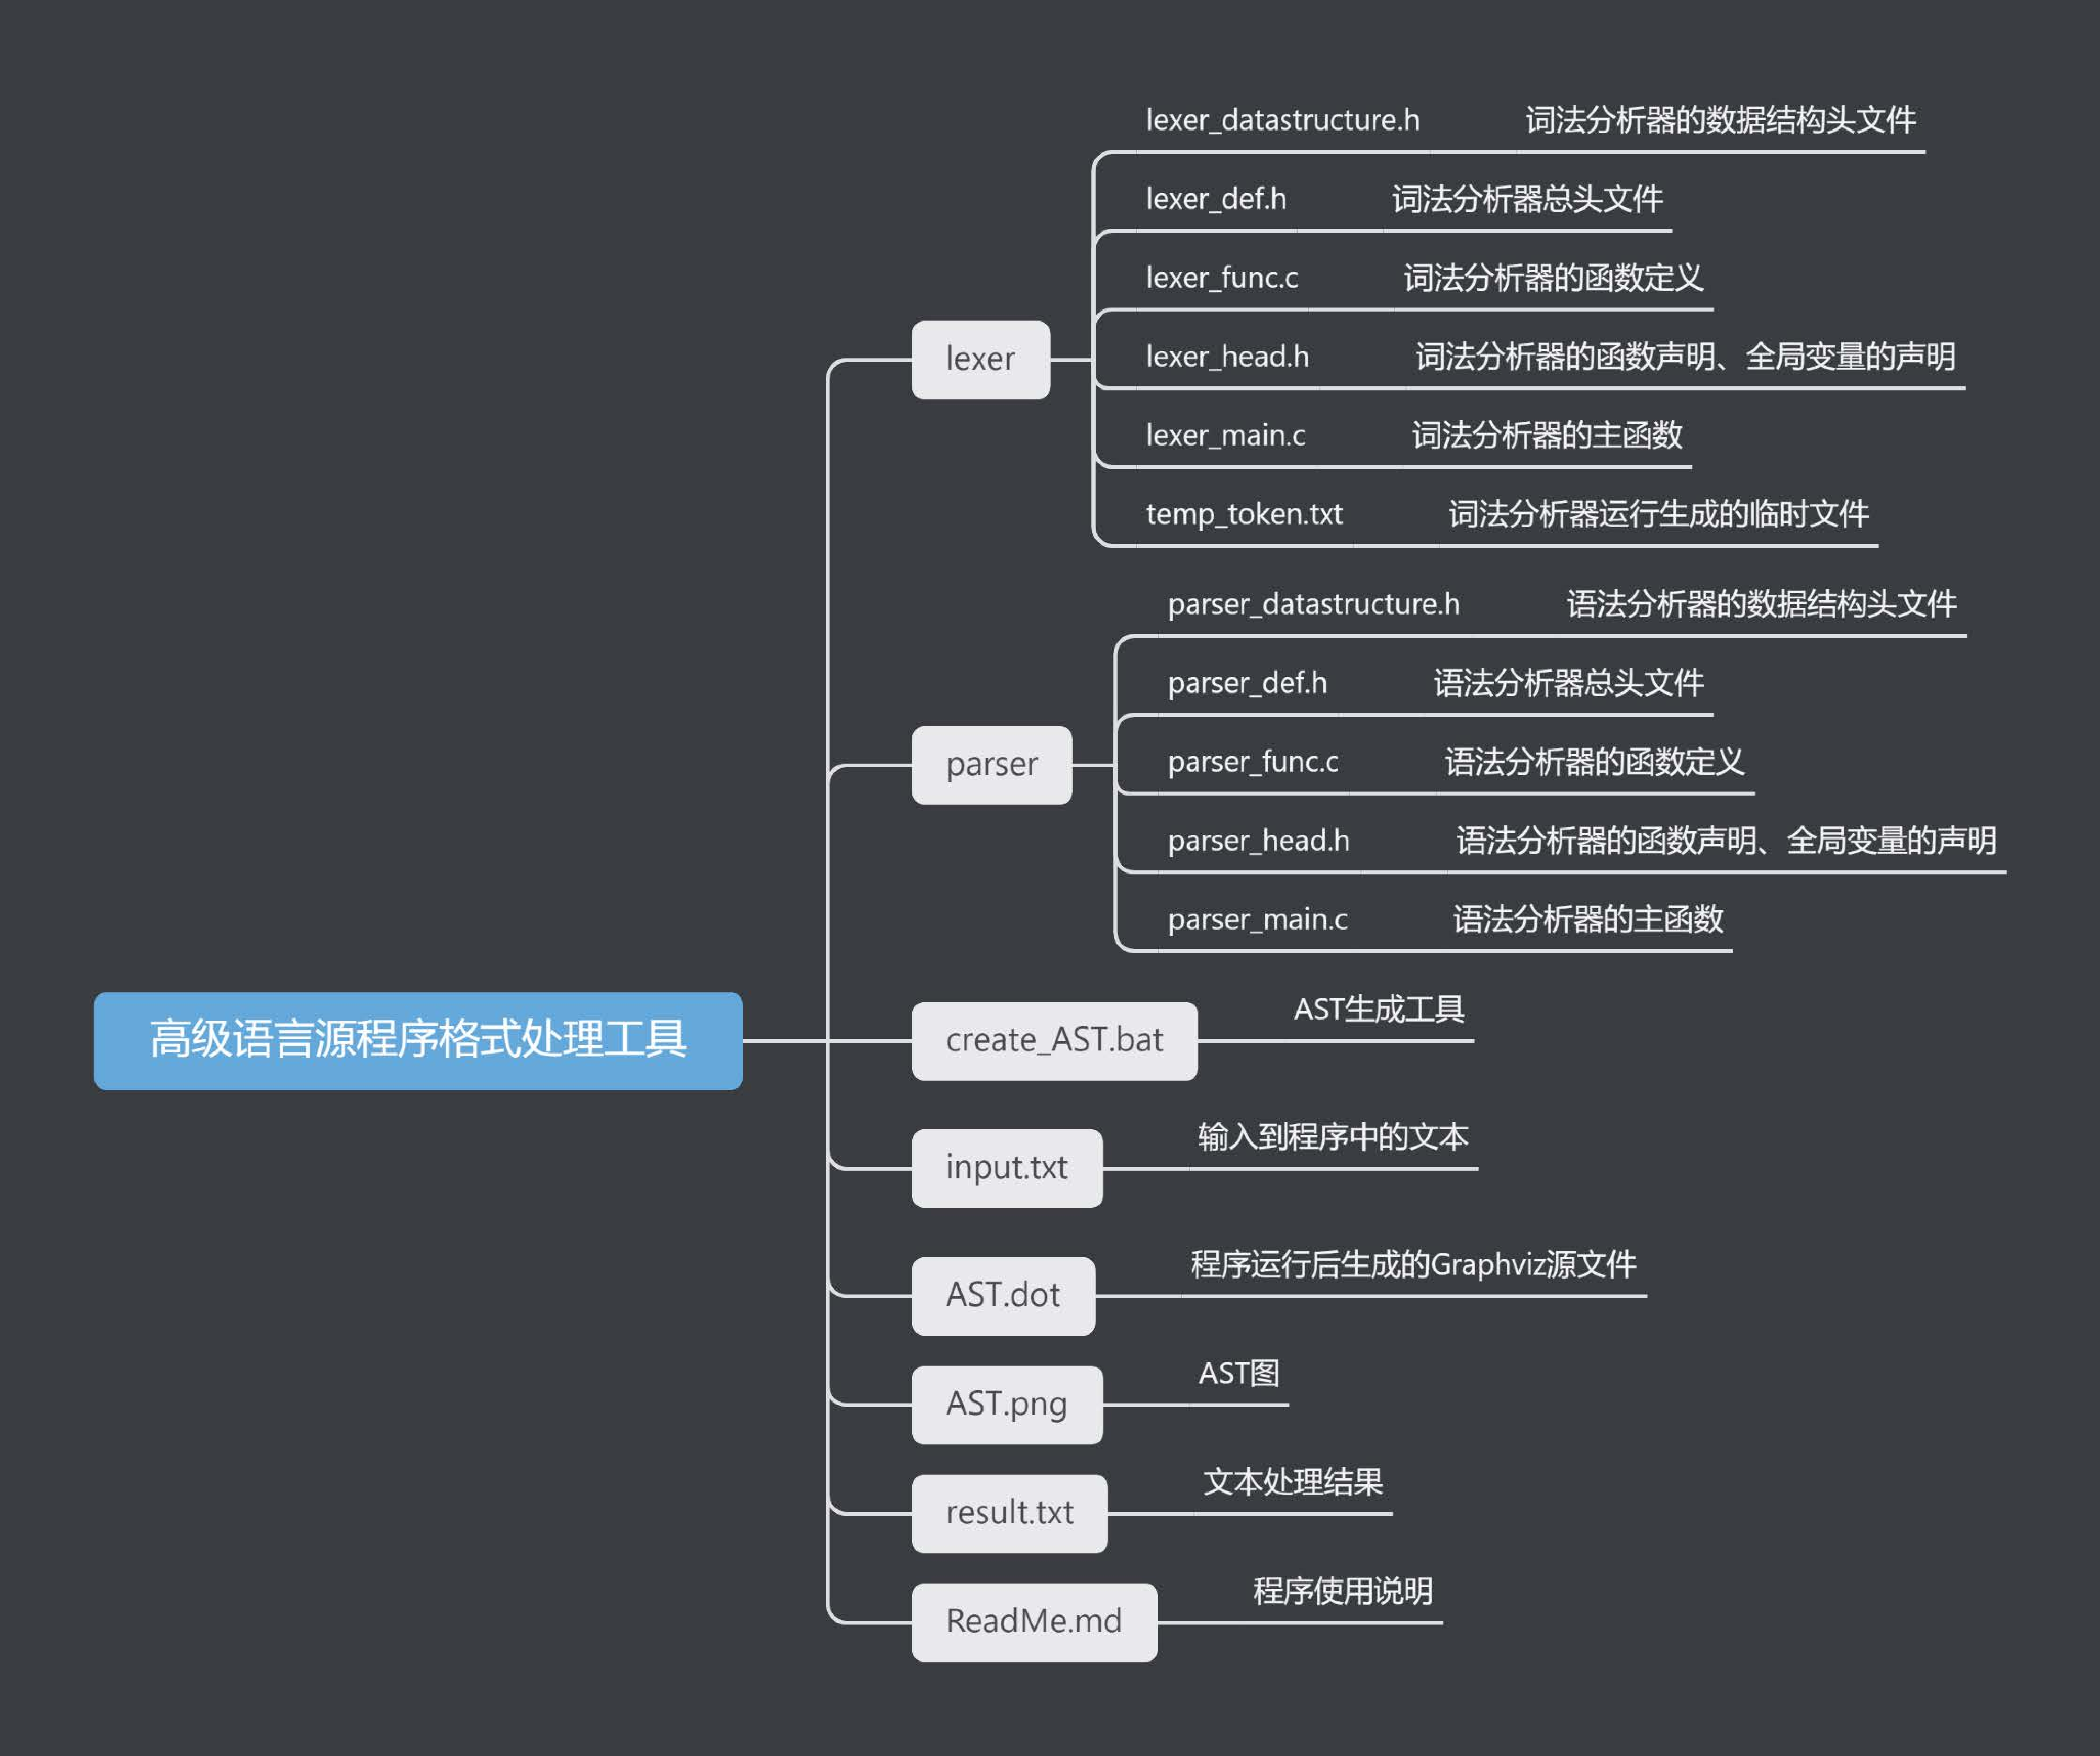
\includegraphics[scale=0.2]{images/高级语言源程序格式处理工具.pdf}
		\caption{程序的文件结构}
		\label{fig1-1}
	\end{center}
\end{figure}

\subsection{词法分析器(lexer)}
程序的词法分析器(lexer)采用C语言编写,负责将输入的字符流处理成词法符号(token)流并输出至temp\_token.txt供语法分析器读取。
与此同时,词法分析器还可以删除输入文本中的注释,找出输入文本的词法错误。

词法分析器的主程序编译运行时,会读入input.txt中的文本,将其处理成词法符号流后写入临时文件temp\_token.txt,
同时在屏幕上打印出所有词法符号的类别和值。如果输入文本有词法错误,词法错误的位置(行号)和出错原因也会被打印在屏幕上。

\subsection{语法分析器(parser)}
程序的语法分析器(lexer)采用C语言编写,负责将输入的词法符号(token)流处理成抽象语法树(AST),生成基于dot语言的抽象语法树信息
并把前序遍历AST(这也是文本处理过程)的结果输出至result.txt。与此同时,语法分析器还可以找出输入文本的语法错误。

语法分析器的主程序编译运行时,会读入temp\_token.txt中的词法符号流,按照C语言子集的文法定义进行递归下降分析,
在分析的过程中进行文本格式的处理和dot代码的生成,并把上述两个结果输出至result.txt和AST.dot中,同时在屏幕上打印出
AST的书目表的表示形式。如果输入文本有语法错误,语法错误的位置(行号)和出错原因也会被打印在屏幕上。

\subsection{AST生成工具}

AST的生成工具采用Batch语言编写,负责调用Graphviz程序将语法分析器生成的dot代码编译成可视化的抽象语法树。
下图所示的是简单代码《Hello World!》的抽象语法树。
\begin{lstlisting}[title =输入的代码,frame=none]
#include<stdio.h>
int main()
{
printf("Hello World!");
}
\end{lstlisting}
\newpage
\begin{figure}[htb]
	\begin{center}
		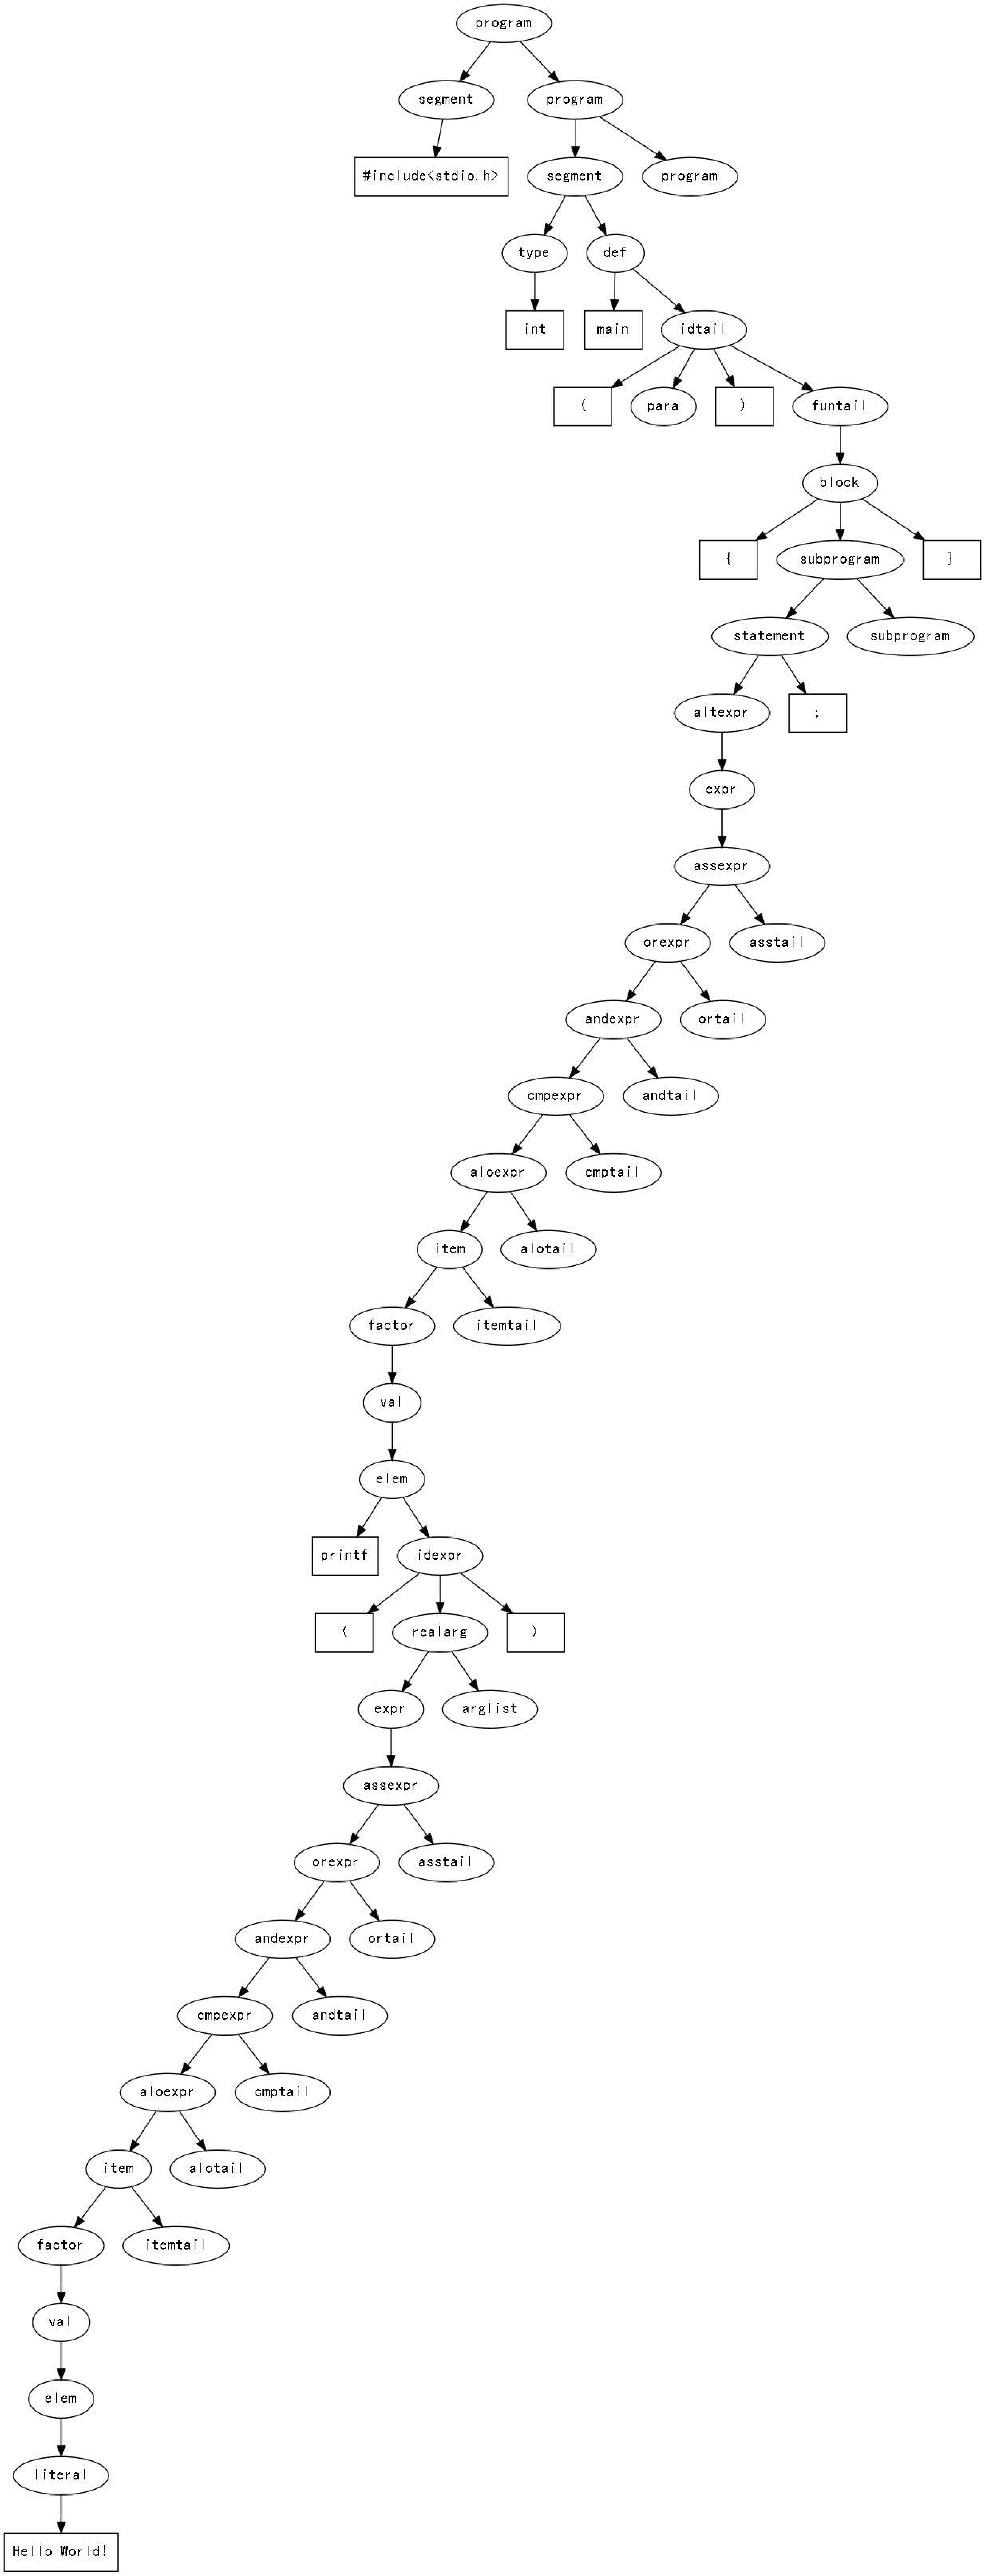
\includegraphics[scale=0.15]{images/HelloWorld.pdf}
		\caption{输出的的AST}
		\label{fig1-2}
	\end{center}
\end{figure}

\newpage
\section{数据结构和算法详细设计}
\subsection{词法分析器(lexer)}
词法分析器采用“硬编码”的方式实现。下面将介绍词法符号的记录和简要的词法分析过程。
\subsubsection{词法符号的记录}
本程序定义了一个枚举类型来表示所有C语言子集支持的词法符号。
C语言子集支持的词法符号主要包括:
\begin{enumerate}
	\item 标识符
	\item 6种数据类型
	\item 不同类型的常量
	\item 逻辑运算
	\item 关系运算
	\item 算术运算
	\item 单目运算
	\item 逗号、冒号等分隔符
	\item 11种语句的关键字
\end{enumerate}
还包括表示出现了词法错误和文件结束的标签。
在进行词法分析的过程中,采用TOKEN结构存储已分析出来的词法符号,其定义如下:
\begin{lstlisting}[title =TOKEN的定义,frame=none]
typedef struct TOKEN//定义token。
{
	int type;//词法符号的类型
	char value[MAXLEN_OF_CONTENT];//词法符号的值
	int loc;//词法符号的位置
}Token;
\end{lstlisting}
同时我们定义了7种词法错误:
\begin{enumerate}
	\item 字符串缺少右双引号
	\item 二进制常量无值
	\item 十六进制常量无值
	\item 字符类型缺少右单引号
	\item 字符常量无值
	\item 逻辑或缺少|
	\item 错误的词法记号
\end{enumerate}
\subsubsection{词法分析的过程}
首先我们进行注释的清除,当扫描到双斜线时,表明行注释开始,开始持续清除字符直到扫描到换行符。
当扫描到连续的斜线和星号时,表明块注释开始,开始持续清除字符直到扫描到块注释结束。

当扫描到\"\#\"时,说明遇到了编译预处理的语句,这时我们新建一个类型为“宏”的词法符号并把值设置成这一行的所有字符。

接着我们进行标识符和关键字的处理,当扫描到下划线或字母时,说明下一个词法符号是标识符或关键字。
我们继续扫描到第一个不是下划线、数字或字母的字符,并存储扫描结果。接着把扫描结果和关键字表比对来确定究竟是
关键字还是标识符。

接着进行常量的判断,对于数字型常量,若以0开头,那么它可能是0或者八进制数;若以0x开头,那么它是十六进制数;若以
0b开头,那么它是二进制数。(标准C语言中并没有二进制常量,这是C语言子集的独有的特性)。字符常量以单引号开头,字符串常量
以双引号开头。

最后进行分隔符和运算符的判断,根据扫描到的结果判断即可。
\subsubsection{词法错误的处理}
当词法分析器不能识别输入的词法符号时,说明输入的文本中出现了词法错误。本程序使用lexerr函数来处理词法错误。
lexerr函数把输入的词法错误符号翻译成提示性语句并和错误出现的位置一起打印到屏幕上。
\subsection{语法分析器(parser)}
我们采用递归下降的方式,根据C语言子集的文法定义进行语法分析。下面介绍C语言子集的文法定义和递归下降分析的过程。
\subsubsection{C语言子集的文法定义}
我们根据如下的文法定义来进行语法分析:
\begin{lstlisting}[title=文法定义,frame=none]
<program>-><segment><program>
<segment>->MAC|EXTERN|<type><def>
<type>->INT|VOID|DOUBLE|CHAR|FLOAT
<def>->*ID<init><deflist>|ID<idtail>
<init>->=<expr>
<deflist>->,<defdata><deflist>|;
<idtail>-><varrdef><deflist>|(<para>)<funtail>
<defdata>->*ID<init>|ID<varrdef>
<varrdef>->[NUM]|<init>
<funtail>->;|<block>
<para>-><type><paradata><paralist>|E
<funtail>->;|<block>
<paradata>->*ID|ID<paradatatail>
<paralist>->,<type><paradata><paralist>|E
<paradatatail>->[NUM]|E
<block>->{<subprogram>}
<expr>-><assexpr>
<subprogram>-><type>ID<varrdef><deflist><subprogram>|<statement><subprogram>|E
<assexpr>-><orexpr><asstail>
<statement>-><altexpr>;|<whilestat>|<forstat>|<dowhilestat>|<ifstat>|BREAK|CONTINUE|RETURN|GETCHAR
<orexpr>-><andexpr><ortail>
<asstail>->=<orexpr><asstail>|E
<altexpr>-><expr>|E
<whilestat>->WHILE(<altexpr>){<block>}
<forstat>->FOR(<altexpr>;<altexpr>;<altexpr>){<block>}
<dowhilestat>->DO<block>WHILE(<altexpr>)
<ifstat>->IF(<expr>)<block><elsestat>
<andexpr>-><cmpexpr><andtail>
<ortail>->OR<andexpr><ortail>|E
<elsestat>->ELSE<block>|E
<cmpexpr>-><aloexpr><cmptail>
<andtail>->AND<cmpexpr><andtail>|E
<aloexpr>-><item><alotail>
<cmptail>-><|>|>=|<=|!=|==<aloexpr><cmptail>|E
<item>-><factor><itemtail>
<alotail>->-|+<item><alotail>|E
<factor>->-|&|--|++<factor>|<val>
<itemtail>->*|%|/<factor><itemtail>|E
<val>-><elem>--|++
<elem>->ID<idexpr>|(<expr>)|<literal>
<idexpr>->[<expr>]|(<realarg>)|E
<literal>->NUM|CHAR|STR
<realarg>-><expr><arglist>|E
<arglist>->,<expr><arglist>|E
\end{lstlisting}

\subsubsection{递归下降分析的过程}
递归下降是对一棵树进行前序遍历的一种方式。我们以文法定义的第一条规则为例来介绍递归下降。
\begin{lstlisting}[title=文法定义的第一条规则,frame=none]
<program>-><segment><program>
\end{lstlisting}
它的含义是从抽象语法树的program节点可以进入segment节点,也可以回到program节点(右递归)。
我们的程序是这样写的
\begin{lstlisting}[title=递归下降的例子,frame=none]
void program()
{
	segment();
	program();
}
\end{lstlisting}
这样在运行时会先进入表示第一个子节点的函数,在进入表示第二个子节点的函数,以此类推,就可以实现抽象语法树的前序遍历。
当函数运行至表示终结符的节点时,我们会判断当前的词法符号和需要的词法符号是否匹配,如果不匹配则需要报告相应的语法错误。
下面的代码是一个处理终结符的例子,表示函数或变量类型的分析(有一些删减):
\begin{lstlisting}[title=type函数中的部分代码,frame=none]
void type()
{
	switch(nexttype)//匹配词法符号
	{
		case INT://INT匹配成功
			gonext();
			break;
		case CHAR://CHAR匹配成功
			gonext();
		default:
			synerr(nexttype,3,INT,CHAR,VOID);//词法符号不匹配,进入语法错误处理函数
			break;
	}
}
\end{lstlisting}
\subsubsection{dot代码的生成和书目表形式的AST的打印}
在前序遍历获得抽象语法树的过程中,我们可以插入控制dot代码生成和打印书目表形式的抽象语法树的代码。

在最后画出的抽象语法树中,我们以长方形节点表示终结符,以椭圆形节点表示非终结符。同时,在节点上标出这个节点的名称。
根据这些要求,我们在程序运行到一个节点的函数内时,首先判断这个节点是否是终结符节点,如果是,那么把这个节点设置成长方形的,
并把这个节点的名称设置成对应的终结符的类型名;如果不是,那么把这个节点设置成椭圆形的,并把这个节点的名称设置成
对应的非终结符的名称,然后在这个节点和所有的子节点连一条有向边。

在书目表形式的打印中,我们使用一个全局变量layer来维护遍历到的AST的层数。使用in函数和out函数使layer变化,表示从当前层
向下进入下一层或向上回溯上一层。我们使用print\_blank函数来打印书目表中的空格,print\_blank读取layer的值,并据此
打印出不同数量的制表位。
\subsubsection{语法错误的处理}
当语法分析器获得了不能匹配的词法符号时,说明发生了语法错误。本程序使用synerr和printerr两个函数来处理语法错误。
printerr的功能相对简单,即输入的语法错误符号翻译成提示性语句并和错误出现的位置一起打印到屏幕上。synerr函数是一个可变参数
的函数,它读取当前出错的词法符号和所有期望中的词法符号。当出错的词法符号的所有可能的前一个符号包含期望中的词法符号之一时,
认为对应的期望中的词法符号缺失,否则认为词法符号错误匹配。
\subsection{AST生成工具}
语法分析器运行后会生成名为AST.dot的dot文件。我们用Batch语言写了一个脚本调用Graphviz编译这个文件并生成最终的
AST.png。其代码如下:
\begin{lstlisting}[title=AST生成工具,frame=none]
@echo off
if not exist 文件所在的文件夹 (
    echo 未找到dot文件夹
    pause
    exit /b 1
) 
cd 文件所在的文件夹
dot -Tpng AST.dot -o AST.png 
if %ERRORLEVEL% NEQ 0 (
    echo 未找到dot文件或graphviz的编译器
    pause
    exit /b 2
)
echo complete
pause
\end{lstlisting}

\newpage

\section{程序实现}

本程序在windows11操作系统下的vscode编辑器中采用C语言、Batch语言开发完成。程序通过MinGW和Graphviz进行编译。
在测试本程序时,首先使用MinGW编译lexer\_main.c,获得并运行lexer\_main.exe。接着使用MinGW编译parser\_main.c,
获得并运行parser\_main.exe。最后在windows11操作系统中运行create\_AST.bat,这个程序自动使用Graphviz编译parser\_main.exe输出的AST.dot,
从而获得AST图和处理后的文本。

需要注意的是,本程序需要配置好Graphviz的编译环境才能够获得AST图,但是Graphviz的编译环境并不影响处理后的文本的输出。

\section{程序测试及结果分析}
我们用5个测试文件进行了程序的测试。测试文件覆盖了绝大部分C语言子集支持的词法符号和语法格式,同时,这些文件的
格式都有待改善。这5个测试程序的名称是:
\begin{enumerate}
	\item Hello World!
	\item 表达式和复杂注释
	\item 各种定义和函数的调用
	\item 各种语句的嵌套
	\item 样例
\end{enumerate}
\subsection{测试文件的内容}
\begin{lstlisting}[title=Hello World!,frame=none]
#include<stdio.h>
int main()
{
printf("Hello World!");
}
\end{lstlisting}

\begin{lstlisting}[title=表达式和复杂注释,frame=none]
//表达式和复杂注释
#include<stdio.h>
int main()
{
int i,j;
i=12;
i=021;
i=0b1;
i=(1%1)+2-3*4/5;
j=/*(1%1)+2-3**/4/5;
///***/
/*//*/
return 0;
}
\end{lstlisting}

\begin{lstlisting}[title=各种定义和函数的调用,frame=none]
/* 各种定义和函数的调用 */
#include<stdio.h>
#include<stdlib.h>
#define A 10
#define F(a,b) a+b
int func1(int a,int b);
int func2(int a,int b)
{return b+a;}
int main()
{
int i=0,j=0,k;
float m=0.5;
double n;
int*p=&i;
int*q;
int arr[15];
k=func1(i,j)+func2(i,j);
return 0;
}
int func1(int a,int b)
{
int c=a+b;
return c;
}
\end{lstlisting}

\begin{lstlisting}[title=各种表达式的嵌套,frame=none]
/* 各种表达式的嵌套 */
#include<stdio.h>
int main()
{int i=0,j=0,k=0;
//if
if(i==0)
{
	if(j==0)
	{
		k=0;
	}
	k=0;
}
if(j==0){k=0;}
else if(j!=0){k=0;}
else{j=0;}
//while
while(i!=0)
{
	while(j!=0)
	{
		k=0;
	}
	k=0;
}
while(j!=0){k=0;}
//for
for(i=0;i<2;i++)
{
	for(int m=4;m>2;m--)
	{
		i=0;
		continue;
	}
}
for(i=0;i<=2;i++){i=0;}
//do-while
do
{
	do
	{
		k=0;
	}while(j!=0);
	k=0;
}while(i!=0);
do{k=0;}
while(j!=0);
//switch-case
switch(i)
{
	case 1:
		i=0;
		break;
	case 2:
		i=1;
		break;
	case 3:
		switch(i){case 1:break;}
	default:
		break;
}
switch(i){case 1:break;}
return 0;
}
\end{lstlisting}

\begin{lstlisting}[title=样例,frame=none]
int i,j;
int fun(int a, float b)
{
int m;
if (a>b) 
m=a;
else 
m=b;
return m;
}
float x,y;
\end{lstlisting}

\subsection{处理后的代码}

\begin{lstlisting}[title=Hello World!,frame=none]
#include<stdio.h>
 int main ( ) 
	
{
	printf ( "Hello World!" ) ;
}
\end{lstlisting}

\begin{lstlisting}[title=表达式和复杂注释,frame=none]
#include<stdio.h>
 int main ( ) 
	
{
	int i , j ;
	i = 12 ;
	i = 21 ;
	i = 1 ;
	i = ( 1 % 1 ) + 2 - 3 * 4 / 5 ;
	j = 4 / 5 ;
	return 0 ;
}
\end{lstlisting}

\begin{lstlisting}[title=各种定义和函数的调用,frame=none]
#include<stdio.h>
 #include<stdlib.h>
 #define A 10
 #define F(a,b) a+b
 int func1 ( int a , int b ) ;
int func2 ( int a , int b ) 
	
{
	return b + a ;
}
int main ( ) 
	
{
	int i = 0 , j = 0 , k ;
	float m = 0.5 ;
	double n ;
	int * p = & i ;
	int * q ;
	int arr [ 15 ] ;
	k = func1 ( i , j ) + func2 ( i , j ) ;
	return 0 ;
}
int func1 ( int a , int b ) 
	
{
	int c = a + b ;
	return c ;
}
\end{lstlisting}

\begin{lstlisting}[title=各种表达式的嵌套,frame=none]
#include<stdio.h>
 int main ( ) 
	
{
	int i = 0 , j = 0 , k = 0 ;
	if ( i == 0 ) 
		
	{
		if ( j == 0 ) 
			
		{
			k = 0 ;
		}
		k = 0 ;
	}
	if ( j == 0 ) 
		
	{
		k = 0 ;
	}
	else 
		if ( j != 0 ) 
		
	{
		k = 0 ;
	}
	else 
		
	{
		j = 0 ;
	}
	while ( i != 0 ) 
		
	{
		while ( j != 0 ) 
			
		{
			k = 0 ;
		}
		k = 0 ;
	}
	while ( j != 0 ) 
		
	{
		k = 0 ;
	}
	for ( i = 0 ; i < 2 ; i ++ ) 
		
	{
		for ( int m = 4 ; m > 2 ; m -- ) 
			
		{
			i = 0 ;
			continue ;
		}
	}
	for ( i = 0 ; i < = = 2 ; i ++ ) 
		
	{
		i = 0 ;
	}
	do 
	{
		do 
		{
			k = 0 ;
		}
		while ( j != 0 ) ;
		k = 0 ;
	}
	while ( i != 0 ) ;
	do 
	{
		k = 0 ;
	}
	while ( j != 0 ) ;
	switch ( i ) 
		
	{
		case 1 :
		  i = 0 ;
		break ;
		case 2 :
		  i = 1 ;
		break ;
		case 3 :
		  switch ( i ) 
			
		{
			case 1 :
			  break ;
		}
		default :
		  break ;
	}
	switch ( i ) 
		
	{
		case 1 :
		  break ;
	}
	return 0 ;
}
\end{lstlisting}

\begin{lstlisting}[title=样例,frame=none]
int i , j ;
int fun ( int a , float b ) 
	
{
	int m ;
	if ( a > b ) 
		m = a ;
	else 
		m = b ;
	return m ;
}
float x , y ;
\end{lstlisting}

\subsection{报错}
为了使错误明显,这里选用较短的程序进行报错测试。

\begin{lstlisting}[title=词法错误:字符串缺少右双引号,frame=none]
#include<stdio.h>
int main()
{
printf("Hello World!);
}
\end{lstlisting}

\begin{figure}[htb]
	\begin{center}
		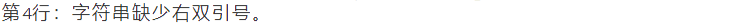
\includegraphics[scale=1]{images/报错1.png}
		\caption{字符串缺少右双引号的报错}
		\label{fig2-1}
	\end{center}
\end{figure}

\begin{lstlisting}[title=词法错误:错误的词法符号,frame=none]
#include<stdio.h>
int main()
{
$
printf("Hello World!");
}
\end{lstlisting}

\begin{figure}[htb]
	\begin{center}
		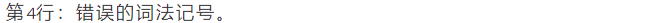
\includegraphics[scale=1]{images/报错3.png}
		\caption{错误的词法符号的报错}
		\label{fig2-2}
	\end{center}
\end{figure}

\begin{lstlisting}[title=语法错误:类型缺失,frame=none]
#include<stdio.h>
main()
{
printf("Hello World!");
}
\end{lstlisting}

\begin{figure}[htb]
	\begin{center}
		
\includegraphics[scale=0.8]{images/报错2.png}
		\caption{类型缺失的报错}
		\label{fig2-3}
	\end{center}
\end{figure}

\begin{lstlisting}[title=语法错误:右小括号缺失,frame=none]
#include<stdio.h>
int main(
{
printf("Hello World!");
}
\end{lstlisting}

\begin{figure}[htb]
	\begin{center}
		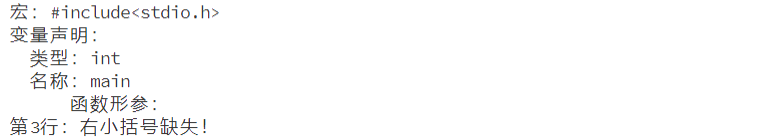
\includegraphics[scale=1]{images/报错4.png}
		\caption{右小括号缺失的报错}
		\label{fig2-4}
	\end{center}
\end{figure}

\begin{lstlisting}[title=语法错误:分号缺失,frame=none]
#include<stdio.h>
int main()
{
printf("Hello World!")
}
\end{lstlisting}

\begin{figure}[htb]
	\begin{center}
		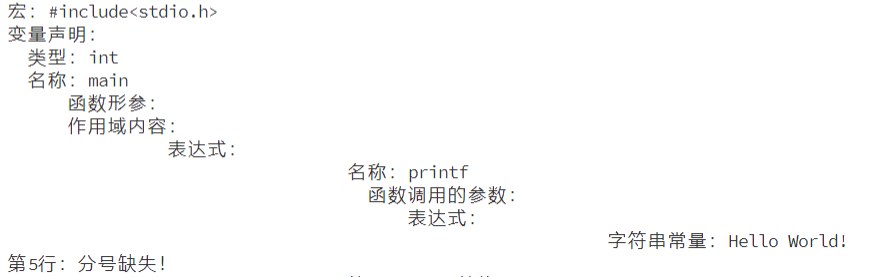
\includegraphics[scale=1]{images/报错5.png}
		\caption{分号缺失的报错}
		\label{fig2-5}
	\end{center}
\end{figure}
	

\subsection{测试程序的AST}
各种表达式的嵌套的图过于大,是分片插入的,完整的图请见附件。
\begin{figure}[htb]
	\begin{center}
		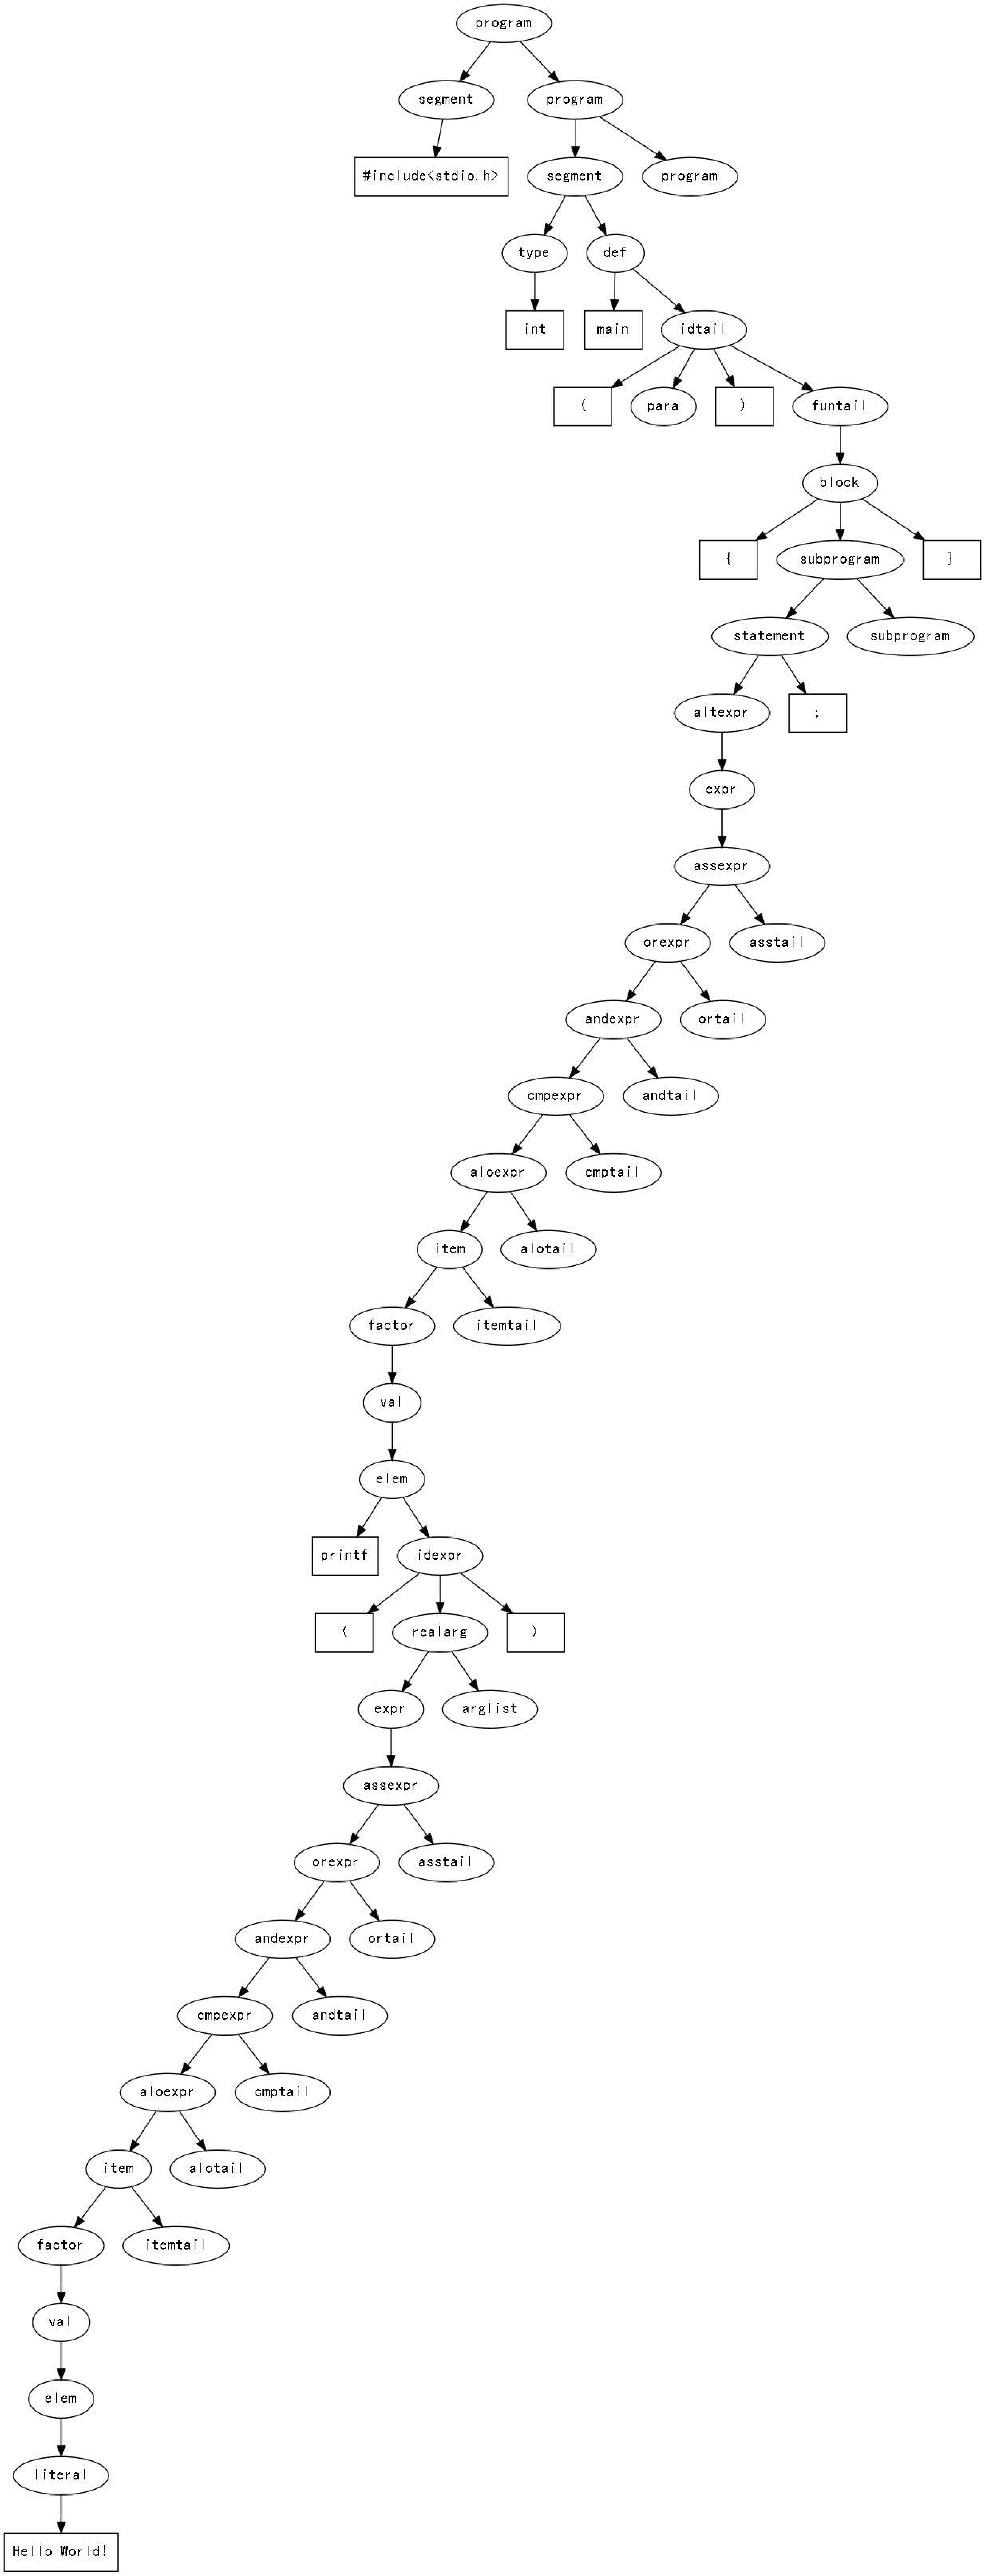
\includegraphics[scale=0.2]{images/HelloWorld.pdf}
		\caption{Hello World!}
		\label{fig3-1}
	\end{center}
\end{figure}
\newpage
\begin{figure}[htb]
	\begin{center}
		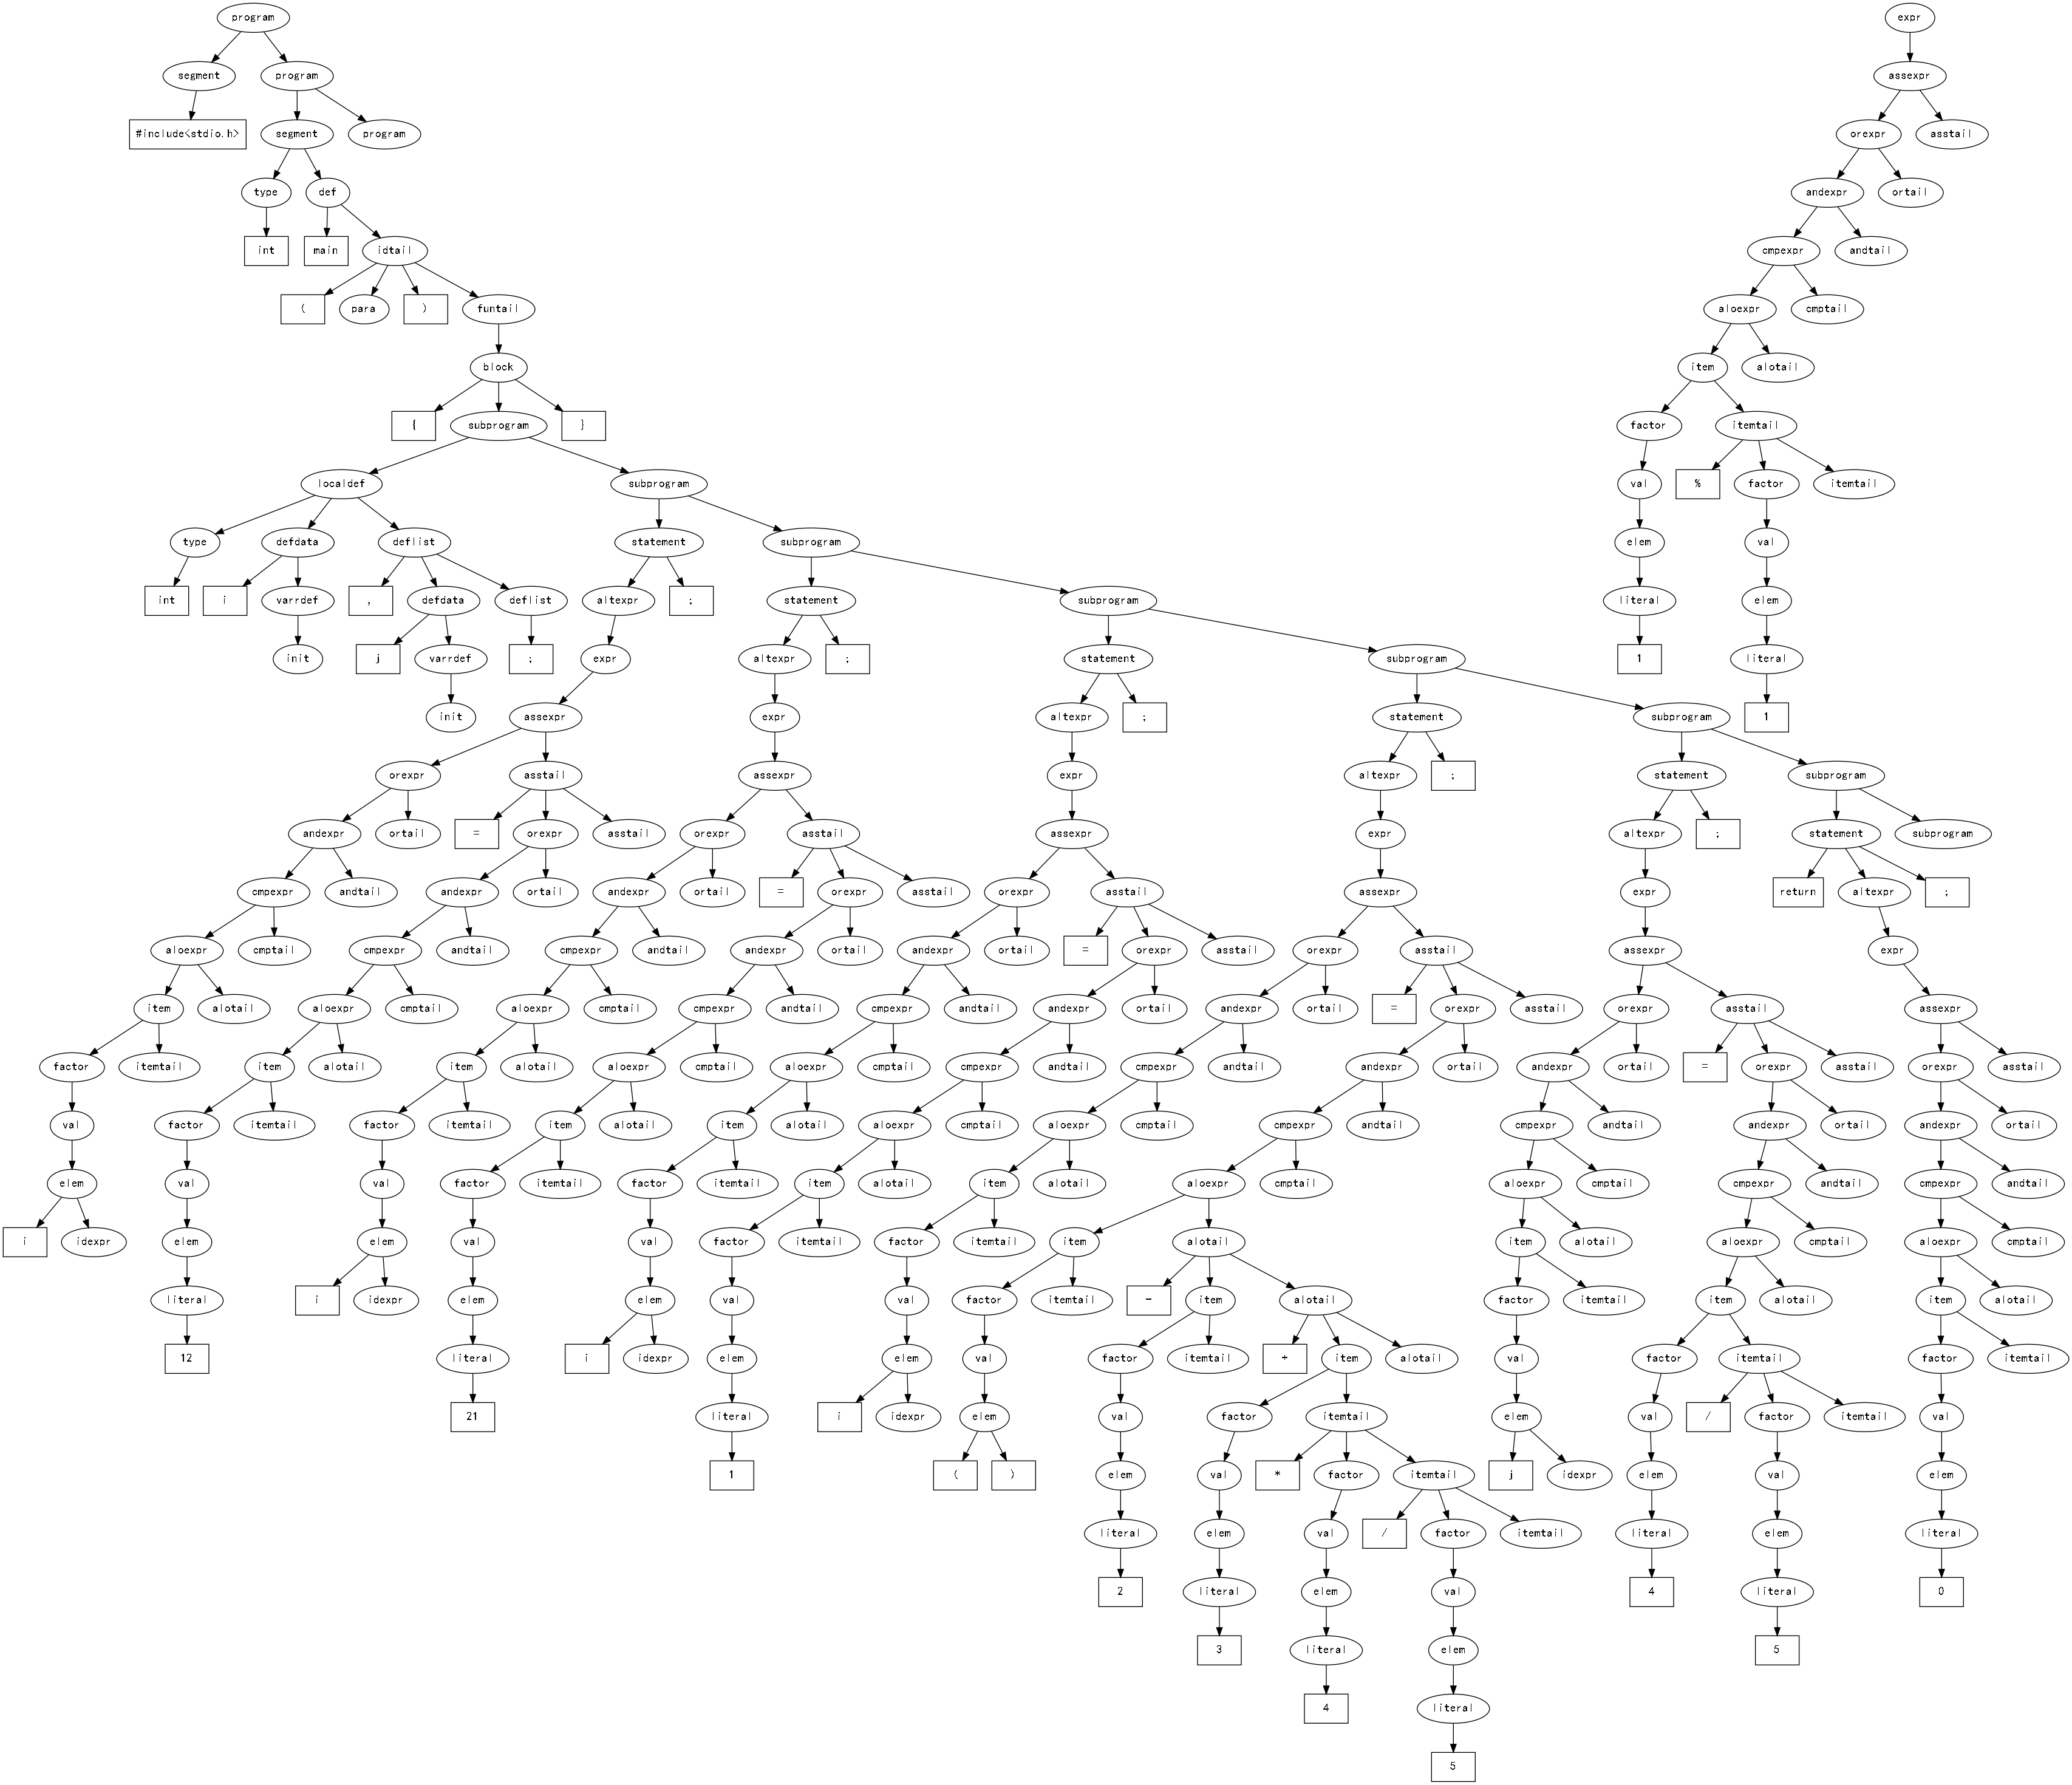
\includegraphics[scale=0.15]{images/表达式和复杂注释.png}
		\caption{表达式和复杂注释}
		\label{fig3-2}
	\end{center}
\end{figure}
\newpage
\begin{figure}[htb]
	\begin{center}
		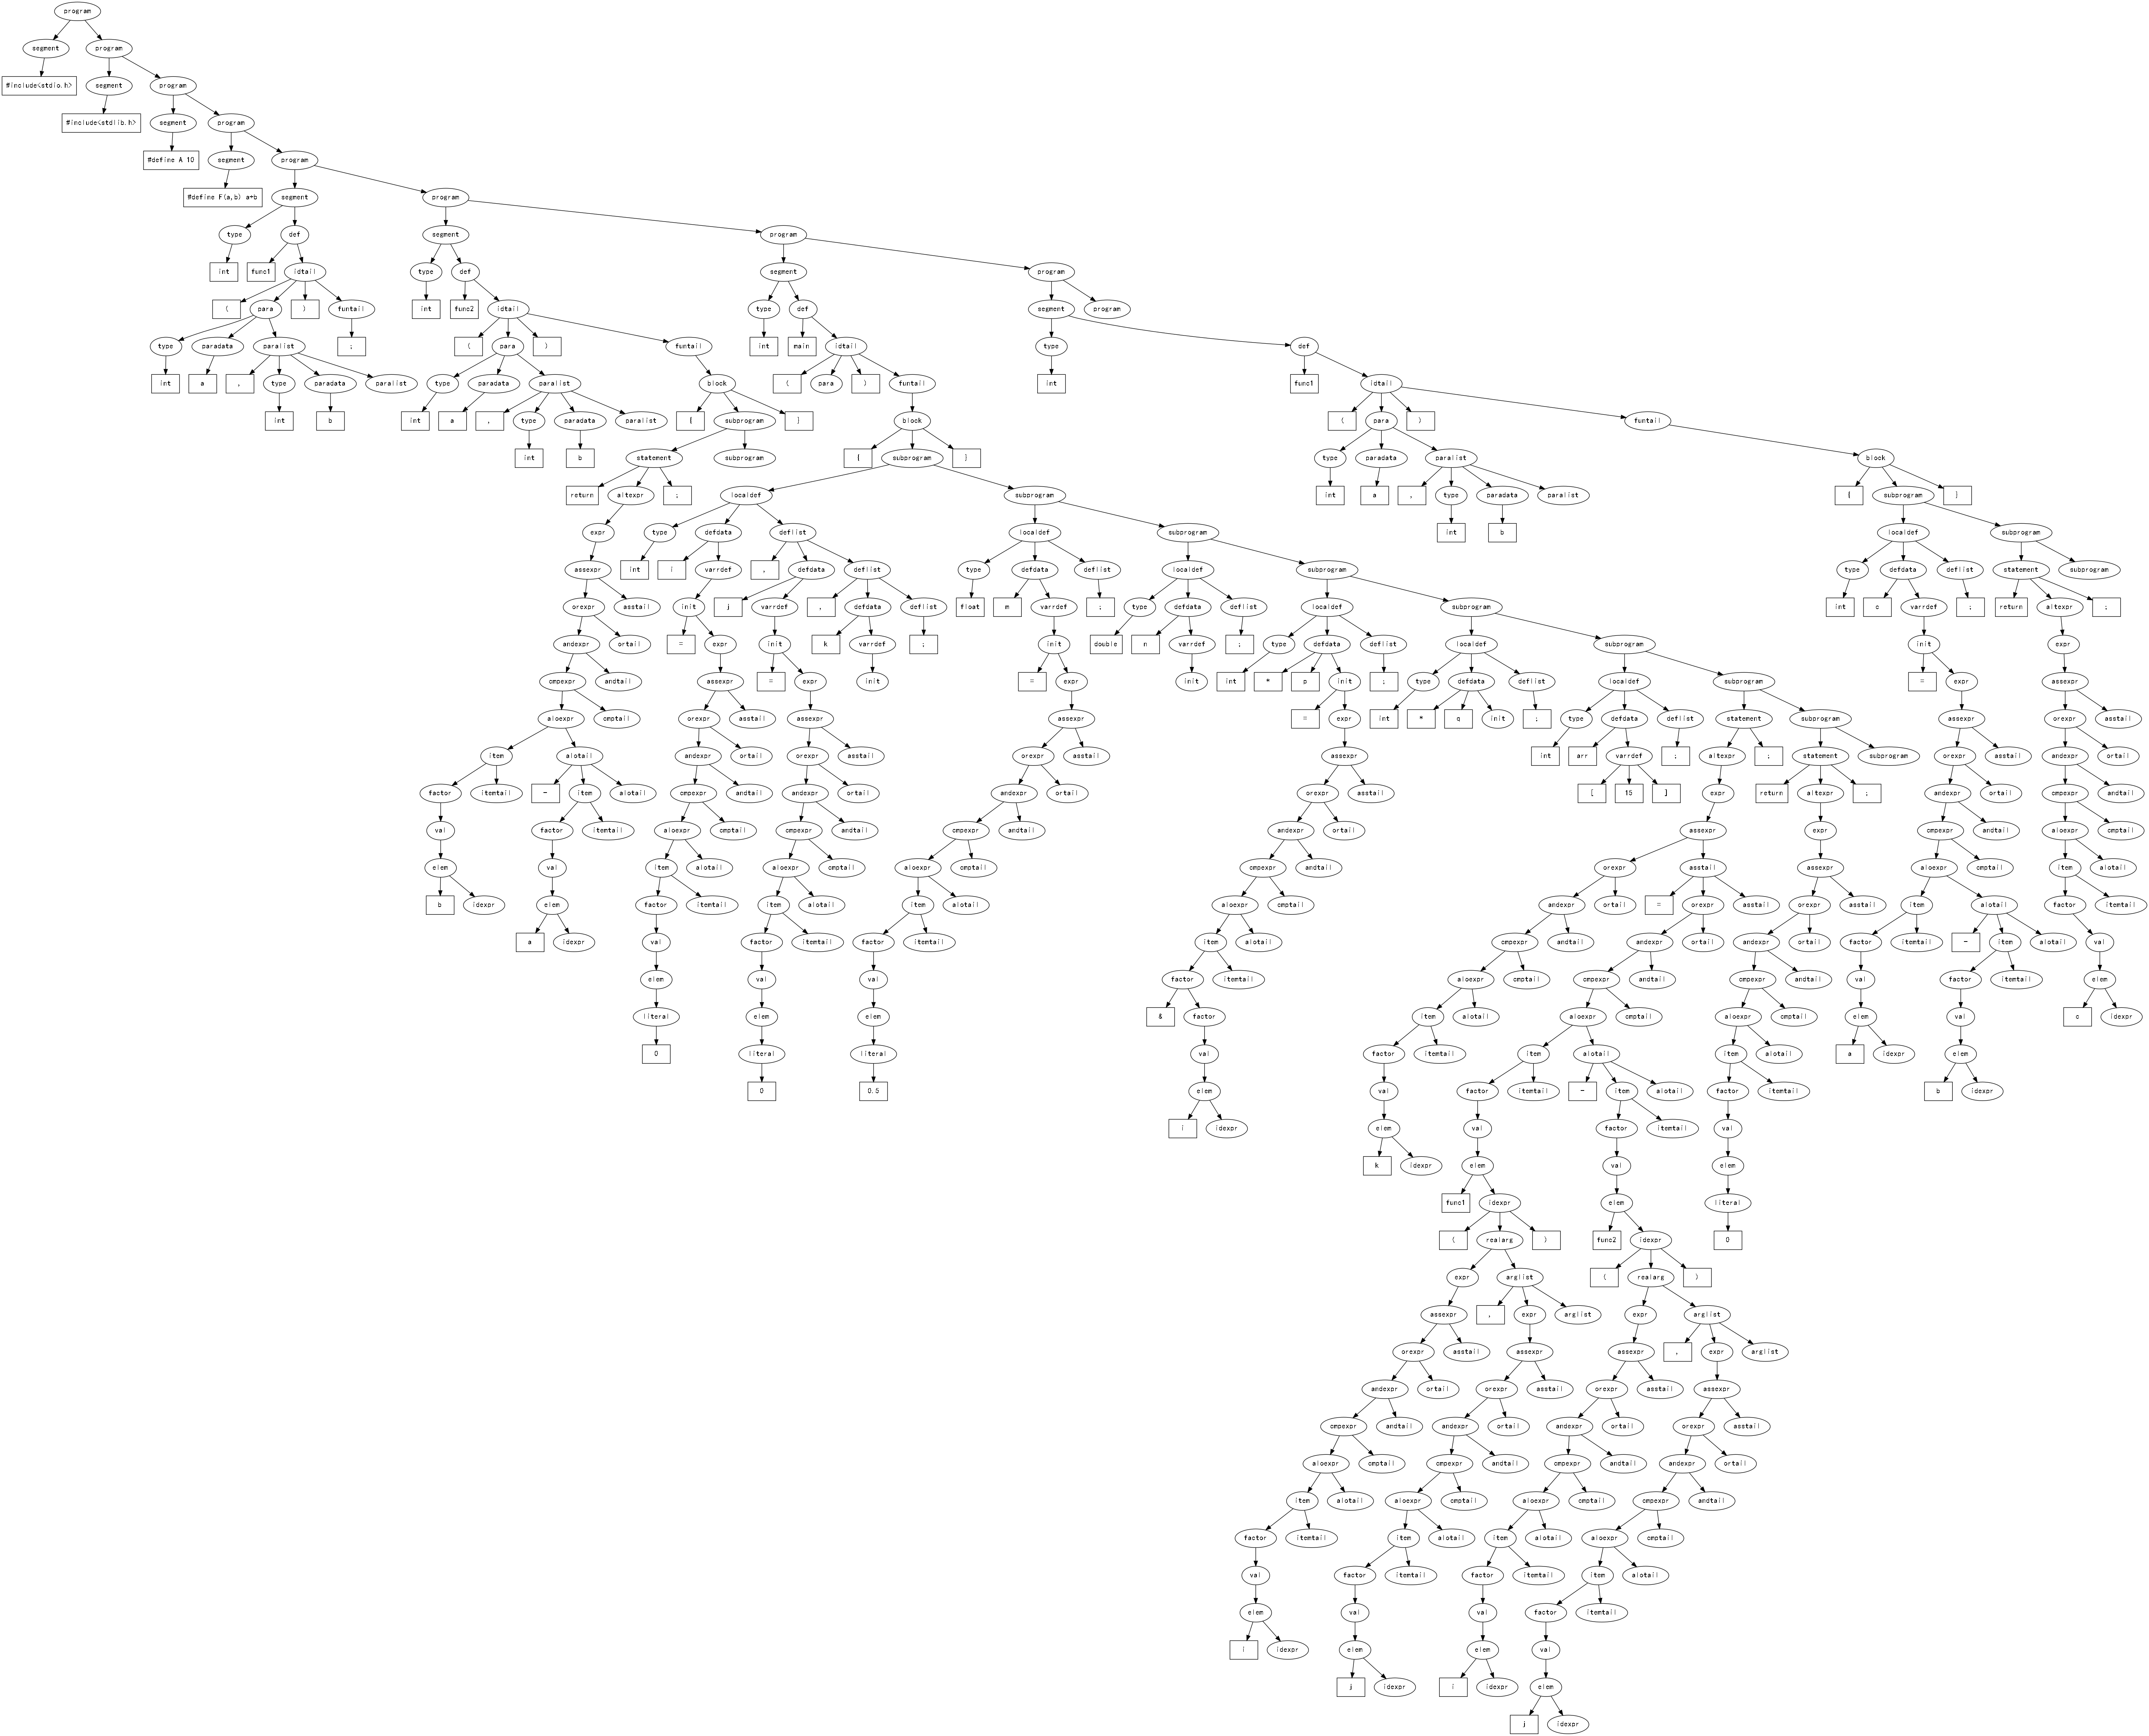
\includegraphics[scale=0.09]{images/各种定义和函数的调用.png}
		\caption{各种定义和函数的调用}
		\label{fig3-3}
	\end{center}
\end{figure}
\newpage

\begin{figure}[htb]
	\begin{center}
		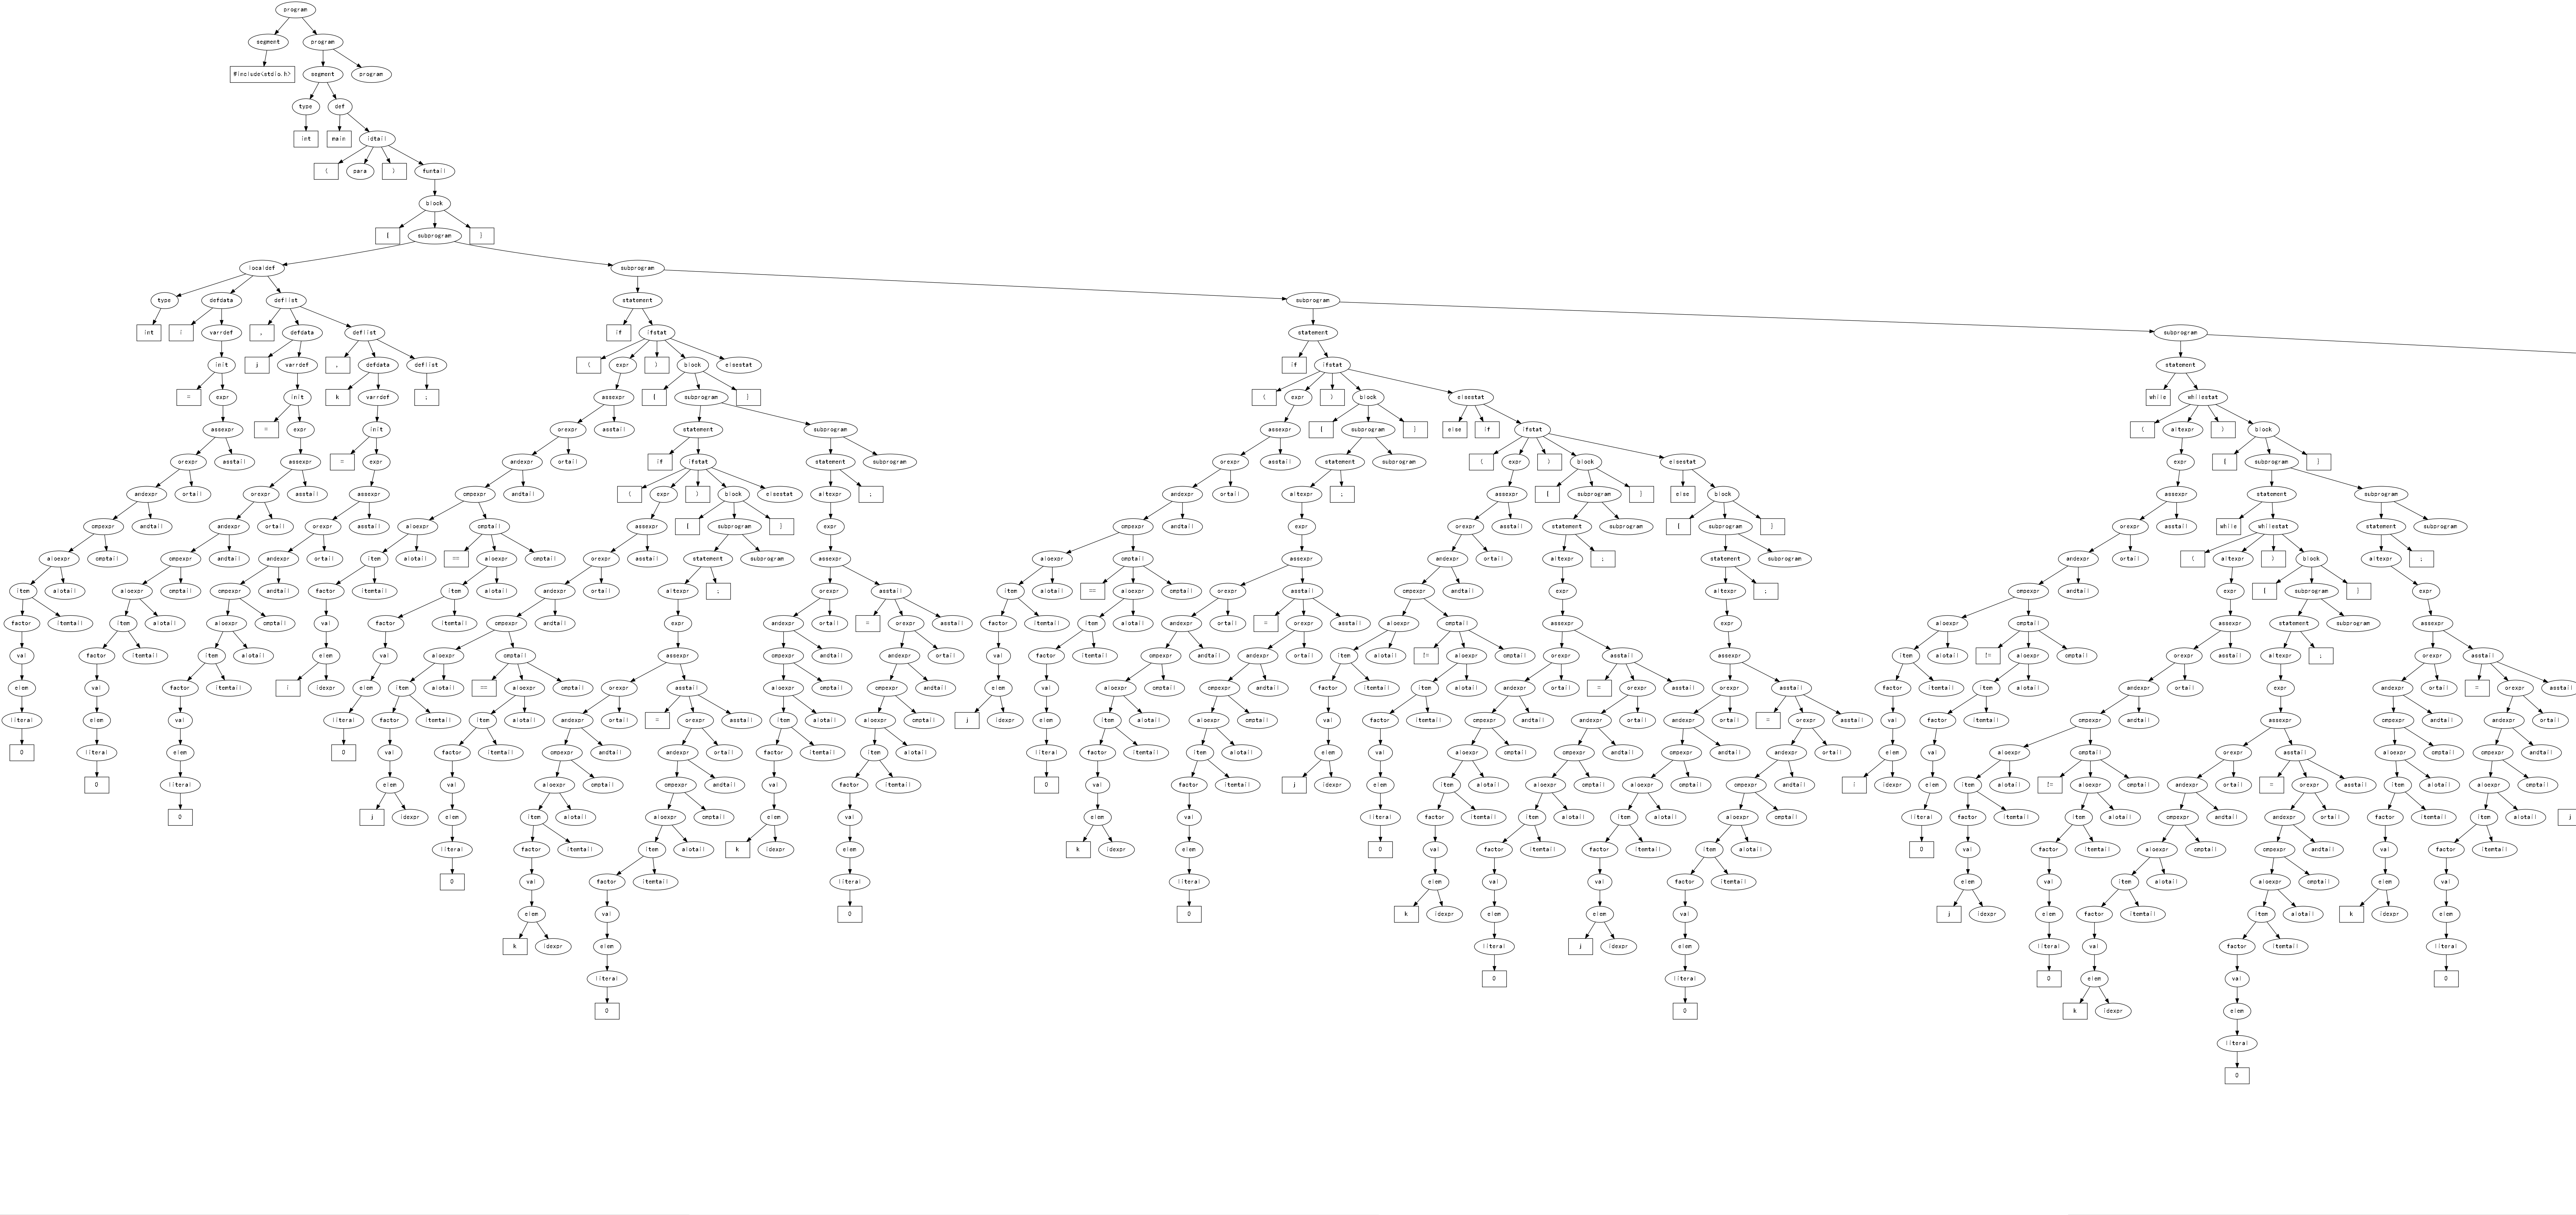
\includegraphics[scale=0.1]{images/各种表达式的嵌套_1.png}
		\caption{各种表达式的嵌套}
		\label{fig3-4}
	\end{center}
\end{figure}
\newpage
\begin{figure}[htb]
	\begin{center}
		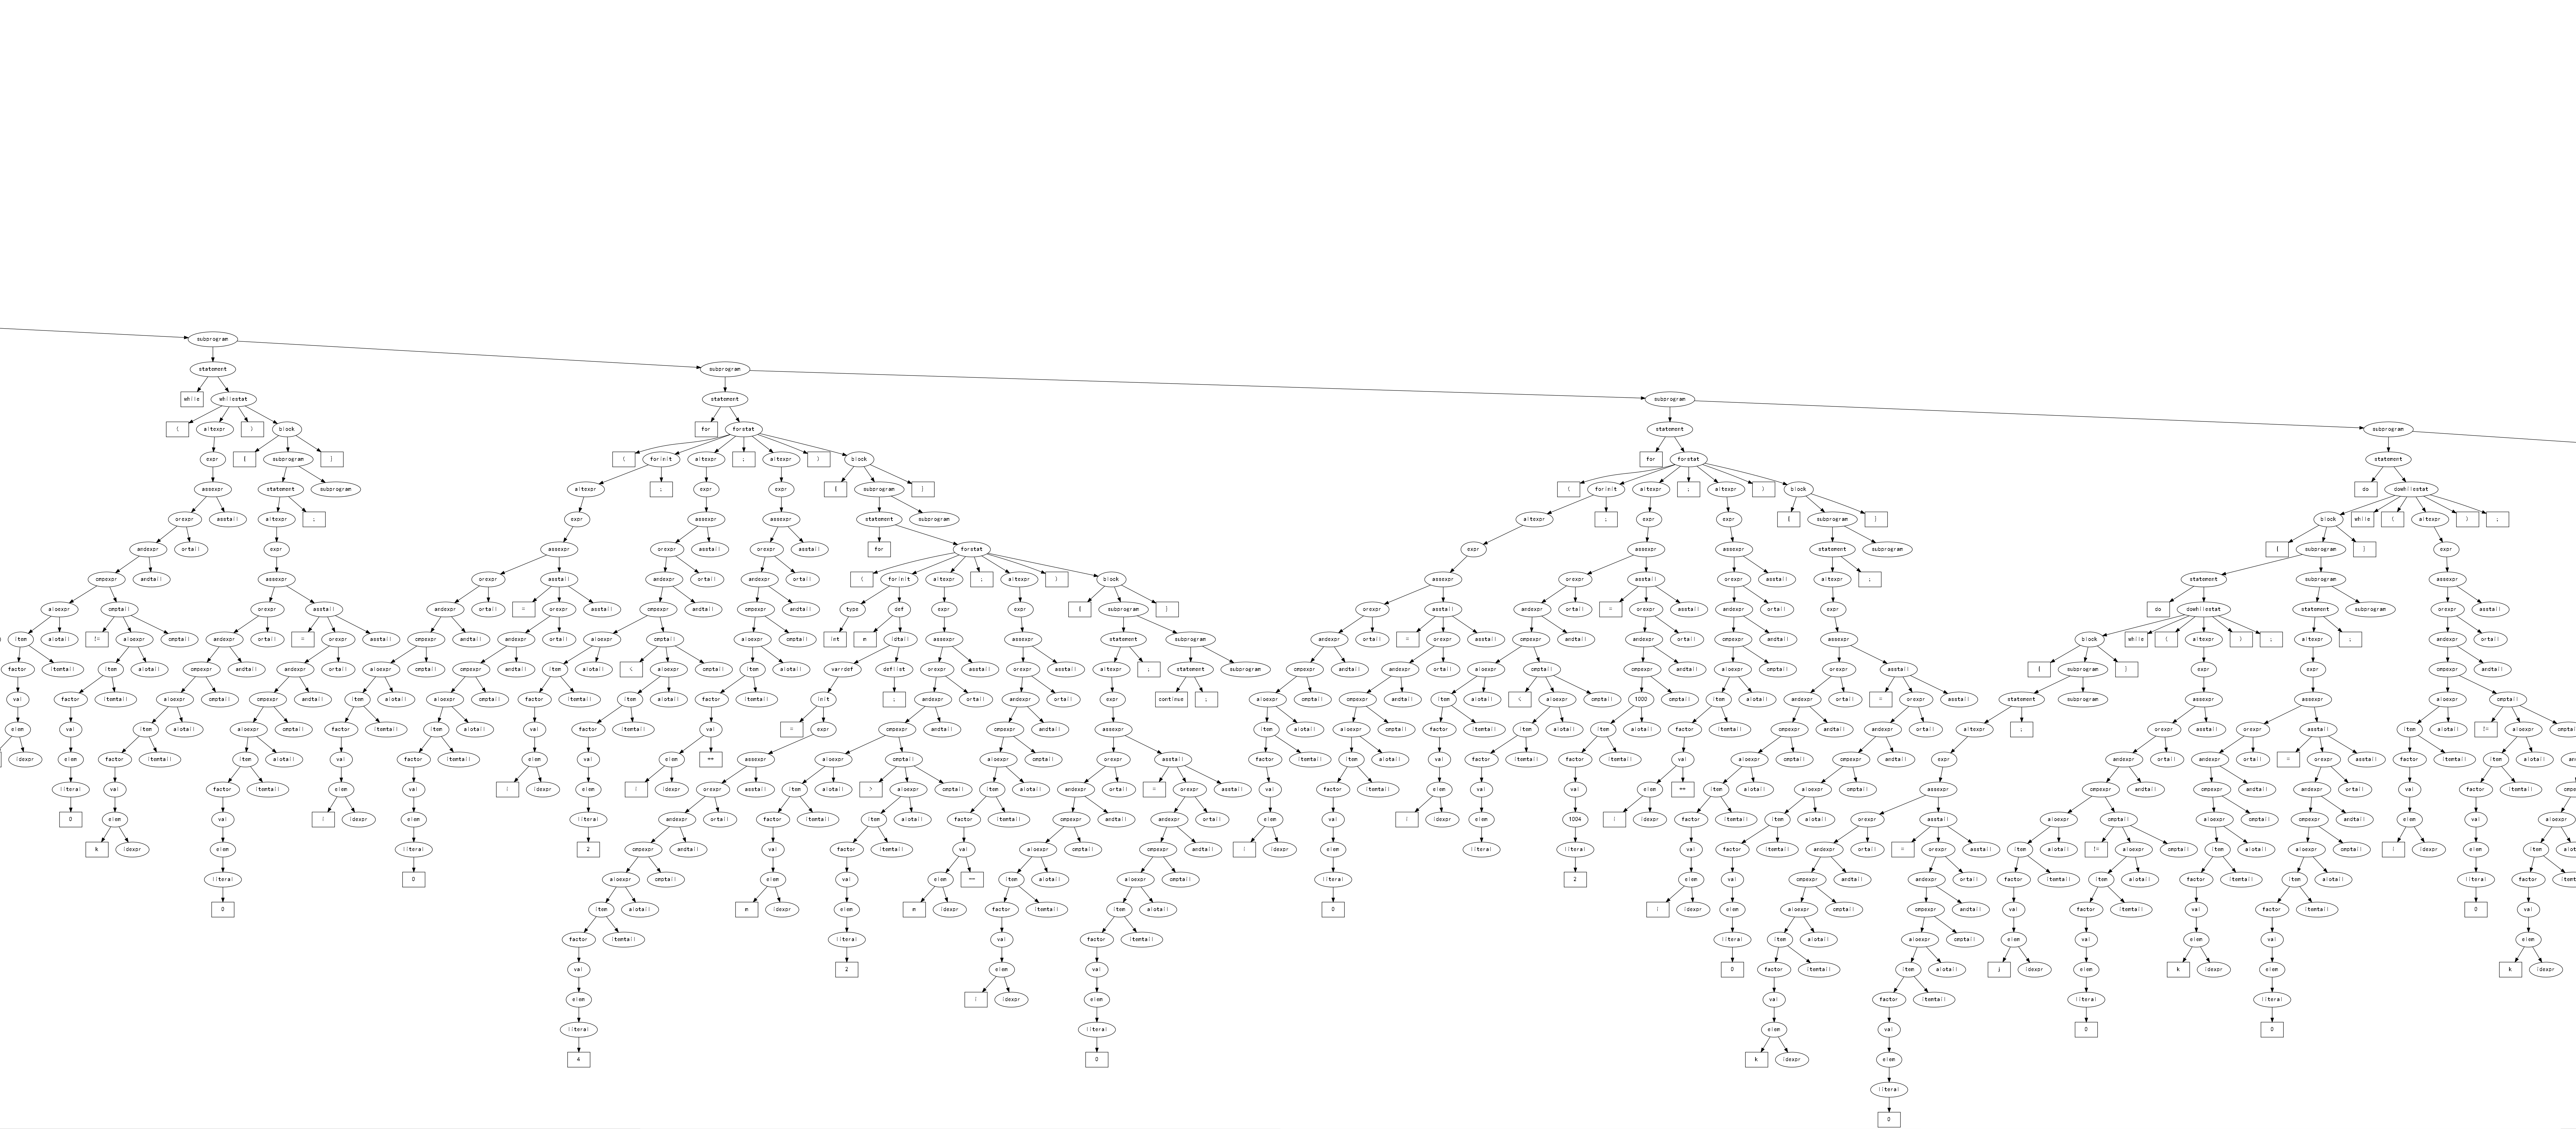
\includegraphics[scale=0.1]{images/各种表达式的嵌套_2.png}
		\caption{各种表达式的嵌套}
		\label{fig3-5}
	\end{center}
\end{figure}
\newpage
\begin{figure}[htb]
	\begin{center}
		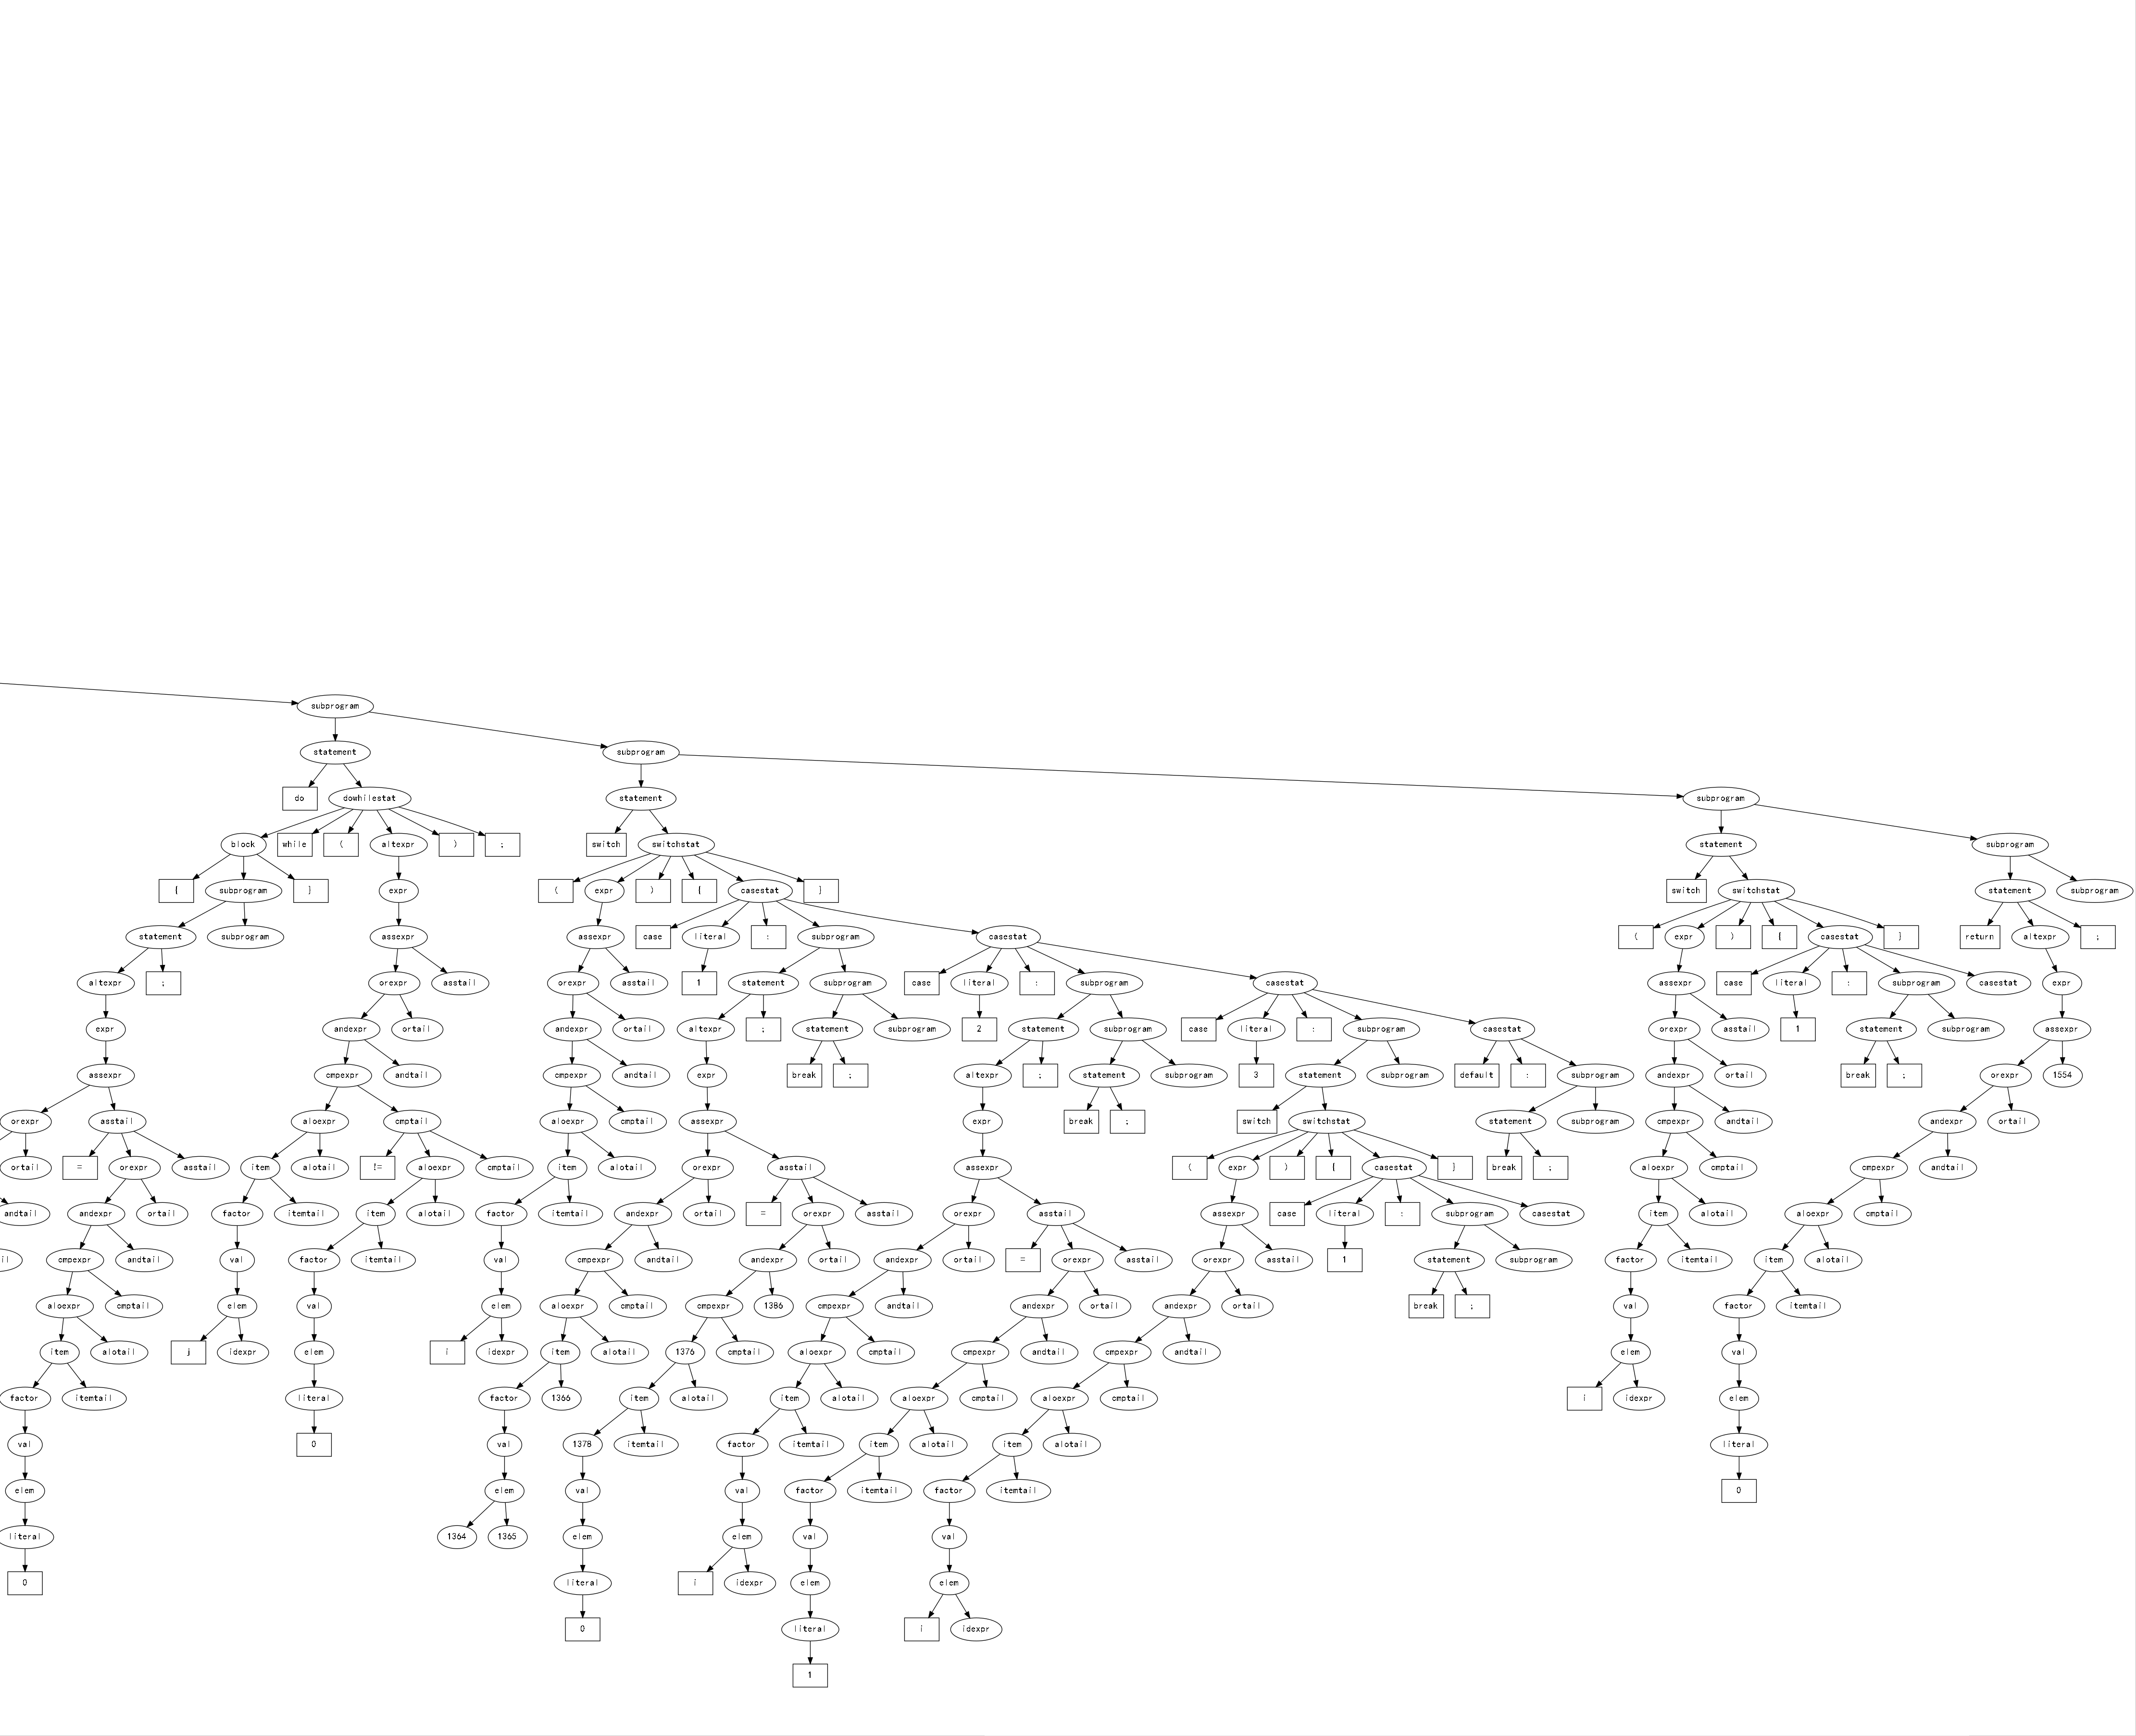
\includegraphics[scale=0.2]{images/各种表达式的嵌套_3.png}
		\caption{各种表达式的嵌套}
		\label{fig3-6}
	\end{center}
\end{figure}
\newpage
\begin{figure}[htb]
	\begin{center}
		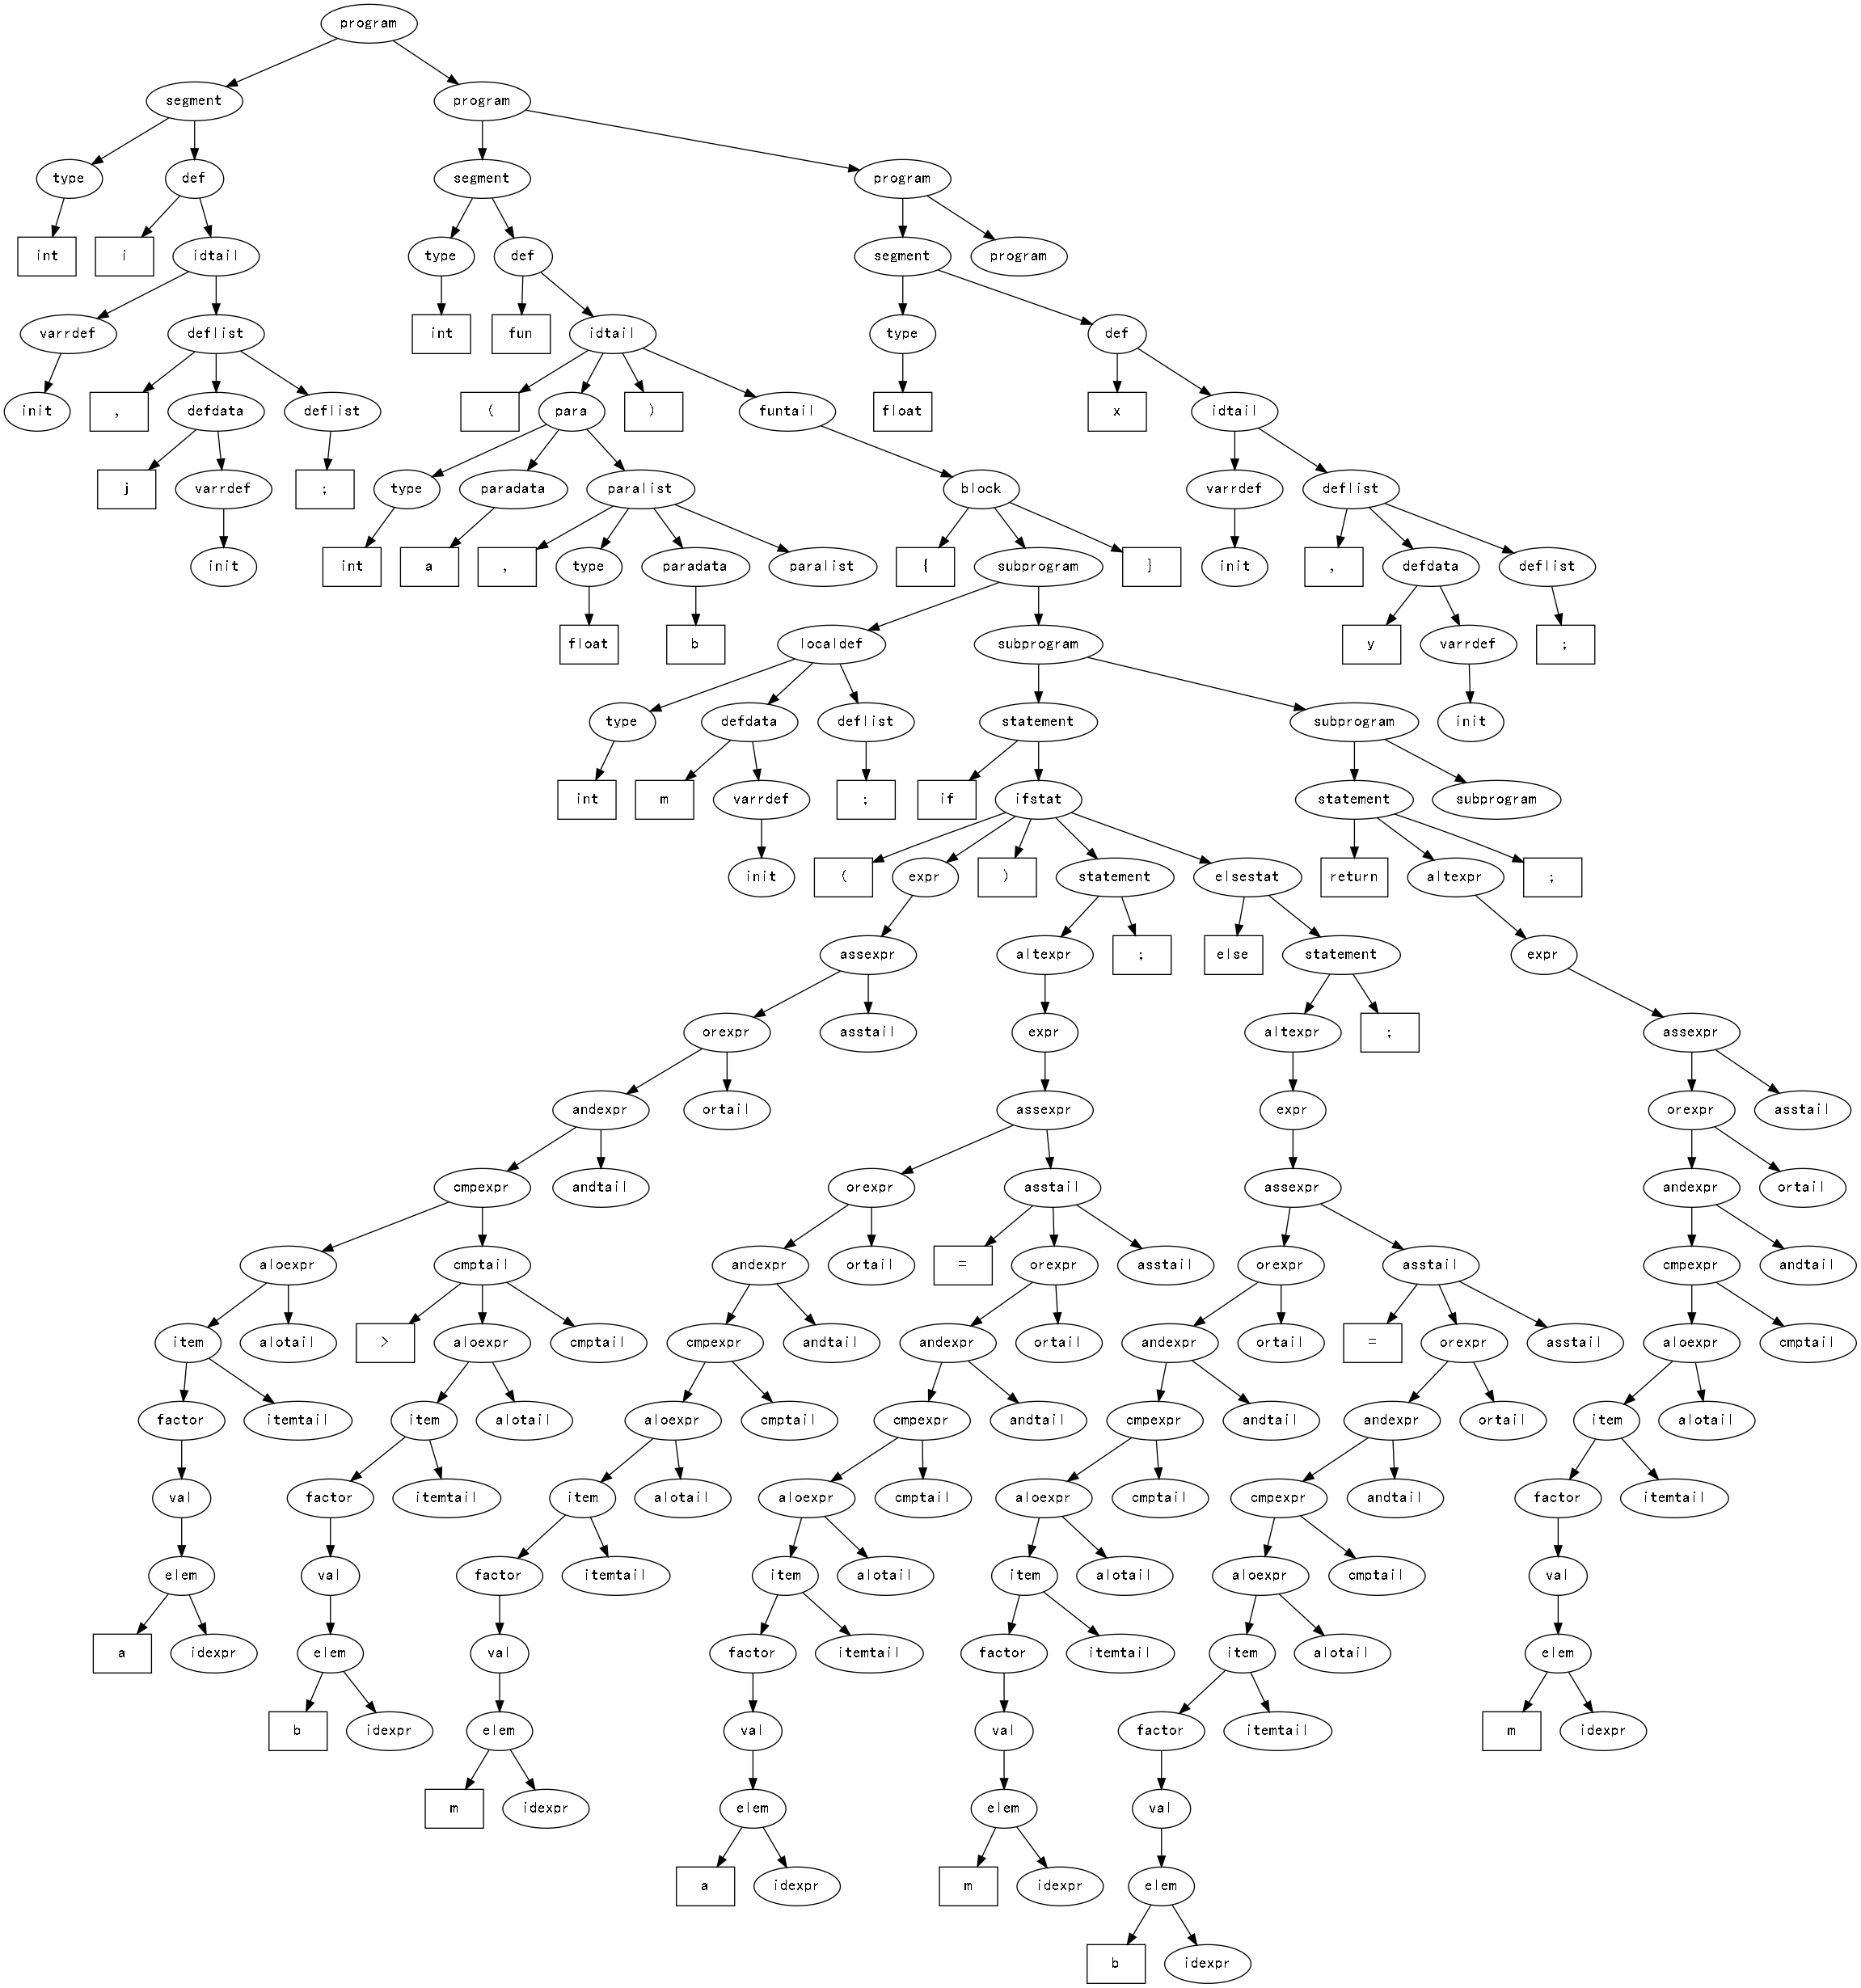
\includegraphics[scale=0.2]{images/样例.png}
		\caption{样例}
		\label{fig3-7}
	\end{center}
\end{figure}
\newpage
\section{复杂度的分析}
本程序采用“硬编码”的方式进行词法分析,采用递归下降的方式进行语法分析,时间复杂度是线性的。

\section{总结、特色与不足}

% \nocite{*} %% 作用是不对文献进行引用,但可以生成文献列表

% \bibliographystyle{Experimental_Report}
% \bibliography{Experimental_Report}
% \setcounter{secnumdepth}{0}
% \appendix
\subsection{高度可视化的抽象语法树}
树的表示方法有书目表法、前中序遍历法等。但这些方法普遍存在着可视化程度低、不直观等缺点。对于很复杂的抽象语法树,
这种缺点尤为突出。本程序采用作图的方式,使用Graphviz把AST画成png格式的图,可以非常直观地描述抽象语法树。
\subsection{更完善的错误处理}
实验要求中对于错误处理仅要求输出词法错误、语法错误的行号,而不要求输出错误原因。这显然对错误的修改不利。
本程序除了可以输出词法错误、语法错误的行号之外,还可以输出错误原因,这样可以使修改错误更容易。
\subsection{无法处理语义错误}
本程序不包含语义分析模块,所以不能处理语义错误。
\newpage
\section{参考文献}
[1] 王生原,董渊,张素琴,吕映芝等. 编译原理(第3版). 北京:清华大学出版社. 前4章


[2] 严蔚敏等.数据结构(C语言版).北京:清华大学出版社

\section{附录A 源程序}
\subsection{词法分析器(lexer)}
\begin{lstlisting}[title=lexer\_datastructure,frame=none]
#ifndef __LEXER_DATASTRUCTURE__
#define __LEXER_DATASTRUCTURE__
typedef struct TOKEN//定义token. 
{
	int type;
	char value[MAXLEN_OF_CONTENT];
	int loc;
}Token;

enum Tag//词法符号的标签 
{
	ERR,//错误。 
	END,//文件结束。 
	ID,//标识符。 
	INT,CHAR,FLOAT,DOUBLE,VOID,EXTERN,//数据类型。 
	NUM,//数字常量。 
	CH,//字符常量。 
	STR,//字符串。 
	NOT,LEA,//!& 
	ADD,SUB,MUL,DIV,MOD,//+-*/% 
	INC,DEC,//++--
	GT,GE,LT,LE,EQU,NEQU,//>>=<<==!=
	AND,OR,//&&|| 
	LPAREN,RPAREN,//() 
	LBRACK,RBRACK,//【】 
	LBRACE,RBRACE,//{} 
	COMMA,COLON,SEMICON,//,:; 
	ASSIGN,//= 
	IF,ELSE,SWITCH,CASE,DEFAULT,WHILE,DO,FOR,BREAK,CONTINUE,RETURN,//关键字。
	MAC//宏。 
}; 

enum LEXERROR//词法错误的标签 
{
	STR_NO_R_QUTION,//字符串缺少右双引号。 
	NUM_BIN_TYPE,//二进制常量无值。 
	NUM_HEX_TYPE,//十六进制常量无值。 
	CHAR_NO_R_QUTION,//字符类型缺少右单引号。 
	CHAR_NO_DATA,//字符常量无值。 
	OR_NO_PAIR,//逻辑或缺少| 。 
	TOKEN_NO_EXIST//错误的词法记号。 
};
#endif 
\end{lstlisting}
\begin{lstlisting}[title=lexer\_def,frame=none]
#ifndef __LEXER_DEF__
#define __LEXER_DEF__
#include<stdio.h>
#include<stdlib.h>
#include<ctype.h>
#include<string.h>
#define MAXLEN_OF_CONTENT 50
#define MAXLEN 1000
#include"lexer_datastructure.h"
#include"lexer_head.h"
#include"lexer_func.c"
#endif
\end{lstlisting}
\begin{lstlisting}[title=lexer\_func,frame=none]
#ifndef __LEXER_FUNC__
#define __LEXER_FUNC__
void wordscanner(FILE*fp,char file[])
{
	int i=0;
	char c;
	while((c=fgetc(fp))!=EOF)
	{
		file[i]=c;
		i++;
	}
	file[i]='\0';
}
int nextstep(char file[],int cnt,char*present,char*next)
{
	*present=*next;
	if(file[cnt]!='\0')
	{
		*next=file[1+cnt];
		return 1;
	}
	else{return 0;}
}
void token_print_to_file(FILE*fp,Token tokenarray[])
{
	int i=0,type=0; 
	if(error==1){return;}//有词法错误,直接返回。
	while((type=tokenarray[i++].type)!=END)
	{
		fprintf(fp,"%d\n",tokenarray[i-1].type);
		if(type==NUM||type==STR||type==ID||type==CH||type==MAC){fprintf(fp,"%s\n",tokenarray[i-1].value);}
		fprintf(fp,"%d\n",tokenarray[i-1].loc);
	}
	fprintf(fp,"%d\n",tokenarray[i-1].type);
	fprintf(fp,"%d",tokenarray[i-1].loc);
}
void token_print_to_stdout(Token tokenarray[])
{
	int i=0,type=0;
	if(error==1){return;}//有词法错误,直接返回。 
	while((type=tokenarray[i].type)!=END)
	{
		i++;
		printf("第%d个词法符号:\n",i);
		switch(type)
		{
			case ID:
				printf("\t种别:标识符\n");
				printf("\t内容:%s\n",tokenarray[i-1].value);
				printf("\t位置: 第%d行\n",tokenarray[i-1].loc);
				break;
			case INT:
				printf("\t种别:整型类型\n");
				printf("\t位置: 第%d行\n",tokenarray[i-1].loc);
				break;
			case CHAR:
				printf("\t种别:字符型类型\n");
				printf("\t位置: 第%d行\n",tokenarray[i-1].loc);
				break;
			case FLOAT:
				printf("\t种别:单精度浮点型类型\n");
				printf("\t位置: 第%d行\n",tokenarray[i-1].loc);
				break;
			case DOUBLE:
				printf("\t种别:双精度浮点型类型\n");
				printf("\t位置: 第%d行\n",tokenarray[i-1].loc);
				break;
			case VOID:
				printf("\t种别:空类型\n");
				printf("\t位置: 第%d行\n",tokenarray[i-1].loc);
				break;
			case EXTERN:
				printf("\t种别:全局变量声明\n");
				printf("\t位置: 第%d行\n",tokenarray[i-1].loc);
				break;
			case NUM:
				printf("\t种别:数值常量\n");
				printf("\t内容:%s\n",tokenarray[i-1].value);
				printf("\t位置: 第%d行\n",tokenarray[i-1].loc);
				break;
			case CH:
				printf("\t种别:字符型常量\n");
				printf("\t内容:%s\n",tokenarray[i-1].value);
				printf("\t位置: 第%d行\n",tokenarray[i-1].loc);
				break;
			case STR:
				printf("\t种别:字符串常量\n");
				printf("\t内容:%s\n",tokenarray[i-1].value);
				printf("\t位置: 第%d行\n",tokenarray[i-1].loc);
				break;
			case NOT:
				printf("\t种别:逻辑非\n");
				printf("\t位置: 第%d行\n",tokenarray[i-1].loc);
				break;
			case LEA:
				printf("\t种别:取地址\n");
				printf("\t位置: 第%d行\n",tokenarray[i-1].loc);
				break;
			case ADD:
				printf("\t种别:加法运算\n");
				printf("\t位置: 第%d行\n",tokenarray[i-1].loc);
				break;
			case SUB:
				printf("\t种别:减法运算\n");
				printf("\t位置: 第%d行\n",tokenarray[i-1].loc);
				break;
			case MUL:
				printf("\t种别:乘法运算\n");
				printf("\t位置: 第%d行\n",tokenarray[i-1].loc);
				break;
			case DIV:
				printf("\t种别:除法运算\n");
				printf("\t位置: 第%d行\n",tokenarray[i-1].loc);
				break;
			case MOD:
				printf("\t种别:取余运算\n");
				printf("\t位置: 第%d行\n",tokenarray[i-1].loc);
				break;
			case INC:
				printf("\t种别:自增运算\n");
				printf("\t位置: 第%d行\n",tokenarray[i-1].loc);
				break;
			case DEC:
				printf("\t种别:自减运算\n");
				printf("\t位置: 第%d行\n",tokenarray[i-1].loc);
				break;
			case GT:
				printf("\t种别:大于\n");
				printf("\t位置: 第%d行\n",tokenarray[i-1].loc);
				break;
			case GE:
				printf("\t种别:大于等于\n");
				printf("\t位置: 第%d行\n",tokenarray[i-1].loc);
				break;
			case LT:
				printf("\t种别:小于\n");
				printf("\t位置: 第%d行\n",tokenarray[i-1].loc);
				break;
			case LE:
				printf("\t种别:小于等于\n");
				printf("\t位置: 第%d行\n",tokenarray[i-1].loc);
				break;
			case EQU:
				printf("\t种别:等于\n");
				printf("\t位置: 第%d行\n",tokenarray[i-1].loc);
				break;
			case NEQU:
				printf("\t种别:不等于\n");
				printf("\t位置: 第%d行\n",tokenarray[i-1].loc);
				break;
			case AND:
				printf("\t种别:逻辑与\n");
				printf("\t位置: 第%d行\n",tokenarray[i-1].loc);
				break;
			case OR:
				printf("\t种别:逻辑或\n");
				printf("\t位置: 第%d行\n",tokenarray[i-1].loc);
				break;
			case LPAREN:
				printf("\t种别:左小括号\n");
				printf("\t位置: 第%d行\n",tokenarray[i-1].loc);
				break;
			case RPAREN:
				printf("\t种别:右小括号\n");
				printf("\t位置: 第%d行\n",tokenarray[i-1].loc);
				break;
			case LBRACK:
				printf("\t种别:左中括号\n");
				printf("\t位置: 第%d行\n",tokenarray[i-1].loc);
				break;
			case RBRACK:
				printf("\t种别:右中括号\n");
				printf("\t位置: 第%d行\n",tokenarray[i-1].loc);
				break;
			case LBRACE:
				printf("\t种别:左大括号\n");
				printf("\t位置: 第%d行\n",tokenarray[i-1].loc);
				break;
			case RBRACE:
				printf("\t种别:右大括号\n");
				printf("\t位置: 第%d行\n",tokenarray[i-1].loc);
				break;
			case COMMA:
				printf("\t种别:逗号\n");
				printf("\t位置: 第%d行\n",tokenarray[i-1].loc);
				break;
			case COLON:
				printf("\t种别:冒号\n");
				printf("\t位置: 第%d行\n",tokenarray[i-1].loc);
				break;
			case SEMICON:
				printf("\t种别:分号\n");
				printf("\t位置: 第%d行\n",tokenarray[i-1].loc);
				break;
			case ASSIGN:
				printf("\t种别:赋值\n");
				printf("\t位置: 第%d行\n",tokenarray[i-1].loc);
				break;
			case IF:
				printf("\t种别:if语句\n");
				printf("\t位置: 第%d行\n",tokenarray[i-1].loc);
				break;
			case ELSE:
				printf("\t种别:else语句\n");
				printf("\t位置: 第%d行\n",tokenarray[i-1].loc);
				break;
			case SWITCH:
				printf("\t种别:switch语句\n");
				printf("\t位置: 第%d行\n",tokenarray[i-1].loc);
				break;
			case CASE:
				printf("\t种别:case语句\n");
				printf("\t位置: 第%d行\n",tokenarray[i-1].loc);
				break;
			case DEFAULT:
				printf("\t种别:default语句\n");
				printf("\t位置: 第%d行\n",tokenarray[i-1].loc);
				break;
			case WHILE:
				printf("\t种别:while语句\n");
				printf("\t位置: 第%d行\n",tokenarray[i-1].loc);
				break;
			case DO:
				printf("\t种别:do语句\n");
				printf("\t位置: 第%d行\n",tokenarray[i-1].loc);
				break;
			case FOR:
				printf("\t种别:for语句\n");
				printf("\t位置: 第%d行\n",tokenarray[i-1].loc);
				break;
			case BREAK:
				printf("\t种别:break语句\n");
				printf("\t位置: 第%d行\n",tokenarray[i-1].loc);
				break;
			case CONTINUE:
				printf("\t种别:continue语句\n");
				printf("\t位置: 第%d行\n",tokenarray[i-1].loc);
				break;
			case RETURN:
				printf("\t种别:return语句\n");
				printf("\t位置: 第%d行\n",tokenarray[i-1].loc);
				break;
			case MAC:
				printf("\t种别:宏\n");
				printf("\t内容:%s\n",tokenarray[i-1].value);
				printf("\t位置: 第%d行\n",tokenarray[i-1].loc);
				break;
		}
	} 
}
void lexerr(int a)
{
	switch(a)
	{
		case STR_NO_R_QUTION:
			printf("第%d行:字符串缺少右双引号。\n",lin);
			break;
		case NUM_BIN_TYPE:
			printf("第%d行:二进制常量无值。\n",lin);
			break;
		case NUM_HEX_TYPE:
			printf("第%d行:十六进制常量无值。 \n",lin);
			break;
		case CHAR_NO_R_QUTION:
			printf("第%d行:字符类型缺少右单引号。\n",lin);
			break;
		case CHAR_NO_DATA:
			printf("第%d行:字符常量无值。\n",lin);
			break;
		case OR_NO_PAIR:
			printf("第%d行:逻辑或缺少|。\n",lin);
			break;
		case TOKEN_NO_EXIST:
			printf("第%d行:错误的词法记号。\n",lin);
			break;
	}
	error=1;
}
#endif
\end{lstlisting}
\begin{lstlisting}[title=lexer\_head,frame=none]
#ifndef __LEXER_HEAD__
#define __LEXER_HEAD__
void wordscanner(FILE*fp,char file[]);//读取文件。 
int nextstep(char file[],int cnt,char*present,char*next);//下一步。
void token_print_to_file(FILE*fp,Token tokenarray[]);//打印词法记号到文件。 
void token_print_to_stdout(Token tokenarray[]);//打印词法记号到stdout。 
void lexerr(int a);//处理词法记号错误。 

const char*keywords[]={"int","char","float","double","void","extern","if","else","switch","case","default","while","do","for","break","continue","return",NULL};//关键字。
int lin=1,error=0; //行号和错误标记 
#endif
\end{lstlisting}
\begin{lstlisting}[title=lexer\_main,frame=none]
#include"lexer_def.h"
int main()
{int i=0,j=0,k=0,exi=0;
char present='0';
char next='0';
char file[MAXLEN];
Token tokenarray[MAXLEN];
FILE*Token=fopen("temp_token.txt","w");
FILE*Code=fopen("../input.txt","r");
if(!Code)
{
	printf("文件打开失败。");
	exit(-1);
}
if(!Token)
{
	printf("文件输出失败。");
	exit(-1);
}
//printf("请输入代码,以^Z结尾。\n");
wordscanner(Code,file);
fclose(Code);
present=next=file[0];
while(nextstep(file,i++,&present,&next)!=0)//等于0则文件结束,跳出循环。
{
	if(present=='	'||present==' '){continue;}
	if(present=='\n')
	{
	    lin++;
		continue;
	}//清除空格和回车。
	else if(present=='/')//清除注释。
	{
		if(next=='/')////型注释。
		{
			while(next!='\n'){nextstep(file,i++,&present,&next);}
			nextstep(file,i++,&present,&next);
		}
		else if(next=='*')///*型注释。 
		{
			while(1)
			{
				nextstep(file,i++,&present,&next);
				if(present=='*'&&next=='/')
				{
					nextstep(file,i++,&present,&next);
					exi=1;//注释结束,跳出循环。 
					break;
				}
			}
			if(exi==1)//注释结束,跳出循环。
			{
				exi=0;
				continue;
			}
		}
		else
		{
			tokenarray[j].type=DIV;
			tokenarray[j].loc=lin;
			j++;
		} 
	}
	else if(present=='#')//判断宏 
	{
		tokenarray[j].type=MAC;
		tokenarray[j].loc=lin;
		j++;
		k=0;
		while((present=='\\'&&next=='\n')||next!='\n')
		{
			tokenarray[j-1].value[k]=present;
			k++;
			nextstep(file,i++,&present,&next);
		}
		tokenarray[j-1].value[k]=present;
		k++;
		tokenarray[j-1].value[k]='\0';
		k=0;
	}
	else if(isalpha(present)!=0||present=='_')//判断是否是标识符。 
	{
		k=0;
		tokenarray[j].type=ID;
		tokenarray[j].loc=lin;
		j++;
		while(isalnum(next)!=0||next=='_')
		{
			tokenarray[j-1].value[k]=present;
			k++;
			nextstep(file,i++,&present,&next);
		}
		tokenarray[j-1].value[k]=present;
		k++;
		tokenarray[j-1].value[k]='\0';
		k=0;
		while(keywords[k]!=NULL)//判断是否是关键字。 
		{
			k++;
			if(strcmp(keywords[k-1],tokenarray[j-1].value)==0)//是,把type设置成相应的关键字。 
			{
				if(k-1<=5){tokenarray[j-1].type=INT+k-1;}
				else{tokenarray[j-1].type=IF+k-7;}
				break;
			}
		}
		k=0;
		continue;
	}
	else if(isdigit(present)!=0)//判断是否是数字常量。 
	{
		tokenarray[j].type=NUM;
		tokenarray[j].loc=lin;
		j++;
		k=0;
		if(present!='0'||(present=='0'&&next=='.'))//判断是否是否是非零十进制数字常量。 
		{
			while(isdigit(next)!=0||next=='.')
			{
				tokenarray[j-1].value[k++]=present;
				nextstep(file,i++,&present,&next);
			}
			tokenarray[j-1].value[k]=present;
			k++;
			tokenarray[j-1].value[k]='\0';
			continue;
		}
		else if(next<='7'&&next>='0')//判断是否是否是非零八进制数字常量。
		{
			nextstep(file,i++,&present,&next);
			while((next<='7'&&next>='0')||next=='.')
			{
				tokenarray[j-1].value[k]=present;
				k++;
				nextstep(file,i++,&present,&next);
			}
			tokenarray[j-1].value[k]=present;
			k++;
			tokenarray[j-1].value[k]='\0';
			continue;
		}
		else if(next=='b')//判断是否是否是非零二进制数字常量。
		{
			nextstep(file,i++,&present,&next);
			if(next!='0'&&next!='1')
			{
				tokenarray[j-1].type=ERR;
			    lexerr(NUM_BIN_TYPE);
			    continue;
			}
			nextstep(file,i++,&present,&next);
			while(next=='0'||next=='1'||next=='.')
			{
				tokenarray[j-1].value[k++]=present;
				nextstep(file,i++,&present,&next);
			}
			tokenarray[j-1].value[k++]=present;
			tokenarray[j-1].value[k]='\0';
			continue;
		}
		else if(next=='x')//判断是否是否是非零十六进制数字常量。
		{
			nextstep(file,i++,&present,&next);
			if(!((next<='F'&&next>='A')||(next>='a'&&next<='f')||isdigit(next)!=0))
			{
				tokenarray[j-1].type=ERR;
			    lexerr(NUM_HEX_TYPE);
			    continue;
			}
			nextstep(file,i++,&present,&next);
			while((next<='F'&&next>='A')||(next>='a'&&next<='f')||isdigit(next)!=0||next=='.')
			{
				tokenarray[j-1].value[k++]=present;
				nextstep(file,i++,&present,&next);
			}
			tokenarray[j-1].value[k++]=present;
			tokenarray[j-1].value[k]='\0';
			continue;
		}
		else//判断是否是零。 
		{
		    tokenarray[j-1].value[0]='0';
		    tokenarray[j-1].value[1]='\0';
		    continue;
		} 
	}
	else if(present=='\'')//判断是否是字符常量。 
	{
		tokenarray[j].type=CH;
		tokenarray[j].loc=lin;
		j++;
		if(next=='\'')
		{
			tokenarray[j-1].type=ERR;
			lexerr(CHAR_NO_DATA);
			continue;
		}
		else
		{
			tokenarray[j-1].value[0]=next;
			tokenarray[j-1].value[1]='\0';
			nextstep(file,i++,&present,&next);
			nextstep(file,i++,&present,&next);
			if(present!='\'')
			{
				tokenarray[j-1].type=ERR;
			    lexerr(CHAR_NO_R_QUTION);
			    while(present!='\''||present!=' '||present!='\n'){nextstep(file,i++,&present,&next);}
			}
			continue;
		}
	}
	else if(present=='"')//判断是否是字符串常量。 
	{
		tokenarray[j].type=STR;
		tokenarray[j].loc=lin;
		j++;
		nextstep(file,i++,&present,&next);
		k=0;
		while(present!='"')
		{
			tokenarray[j-1].value[k++]=present;
			nextstep(file,i++,&present,&next);
			if(present=='\n')
			{
				tokenarray[j-1].type=ERR;
				lexerr(STR_NO_R_QUTION);
				break;
			}
		}
		tokenarray[j-1].value[k]='\0';
		continue;
	}
	else//判断分隔符和运算符。 
	{
		switch(present)
		{
			case '+':
				tokenarray[j].type=ADD;
				tokenarray[j].loc=lin;
				j++;
				if(next=='+')
				{
					tokenarray[j-1].type=INC;
					nextstep(file,i++,&present,&next);
				}
				break;
			case '-':
				tokenarray[j].type=SUB;
				tokenarray[j].loc=lin;
				j++;
				if(next=='-')
				{
					tokenarray[j-1].type=DEC;
					nextstep(file,i++,&present,&next);
				}
				break;
			case '*':
				tokenarray[j].type=MUL;
				tokenarray[j].loc=lin;
				j++;
				break;
			case '/':
				tokenarray[j].type=DIV;
				tokenarray[j].loc=lin;
				j++;
				break;
			case '%':
				tokenarray[j].type=MOD;
				tokenarray[j].loc=lin;
				j++;
				break;
			case '>':
				tokenarray[j].type=GT;
				tokenarray[j].loc=lin;
				j++;
				if(next=='=')
				{
					tokenarray[j-1].type=GE;
					nextstep(file,i++,&present,&next);
				}
				break;
			case '<':
				tokenarray[j].type=LT;
				tokenarray[j].loc=lin;
				j++;
				if(next=='-')
				{
					tokenarray[j-1].type=LE;
					nextstep(file,i++,&present,&next);
				}
				break;
			case '=':
				tokenarray[j].type=ASSIGN;
				tokenarray[j].loc=lin;
				j++;
				if(next=='=')
				{
					tokenarray[j-1].type=EQU;
					nextstep(file,i++,&present,&next);
				}
				break;
			case '&':
				tokenarray[j].type=LEA;
				tokenarray[j].loc=lin;
				j++;
				if(next=='&')
				{
					tokenarray[j-1].type=AND;
					nextstep(file,i++,&present,&next);
				}
				break;
			case '|':
				if(next=='|')
				{
					tokenarray[j].type=OR;
					tokenarray[j].loc=lin;
					j++;
					nextstep(file,i++,&present,&next);
				}
				else
				{
					tokenarray[j++].type=ERR;
					lexerr(OR_NO_PAIR);
				}
				break;
			case '!':
				tokenarray[j].type=NOT;
				tokenarray[j].loc=lin;
				j++;
				if(next=='=')
				{
					tokenarray[j-1].type=NEQU;
					nextstep(file,i++,&present,&next);
				}
				break;
			case ',':
				tokenarray[j].type=COMMA;
				tokenarray[j].loc=lin;
				j++;
				break;
			case ':':
				tokenarray[j].type=COLON;
				tokenarray[j].loc=lin;
				j++;
				break;
			case ';':
				tokenarray[j].type=SEMICON;
				tokenarray[j].loc=lin;
				j++;
				break;
			case '(':
				tokenarray[j].type=LPAREN;
				tokenarray[j].loc=lin;
				j++;
				break;
			case ')':
				tokenarray[j].type=RPAREN;
				tokenarray[j].loc=lin;
				j++;
				break;
			case '[':
				tokenarray[j].type=LBRACK;
				tokenarray[j].loc=lin;
				j++;
				break;
			case ']':
				tokenarray[j].type=RBRACK;
				tokenarray[j].loc=lin;
				j++;
				break;
			case '{':
				tokenarray[j].type=LBRACE;
				tokenarray[j].loc=lin;
				j++;
				break;
			case '}':
				tokenarray[j].type=RBRACE;
				tokenarray[j].loc=lin;
				j++;
				break;
			default:
				tokenarray[j++].type=ERR;
				lexerr(TOKEN_NO_EXIST);
				break;
		}
	}
}
tokenarray[j].type=END;
tokenarray[j].loc=lin;
token_print_to_stdout(tokenarray);
token_print_to_file(Token,tokenarray);
fclose(Token);
return 0; 
}
\end{lstlisting}
\subsection{语法分析器(parser)}
\begin{lstlisting}[title=parser\_datastructure,frame=none]
#ifndef __PARSER_DATASTRUCTURE__
#define __PARSER_DATASTRUCTURE__
typedef struct TOKEN//定义token. 
{
	int type;
	char value[MAXLEN_OF_CONTENT];
	int loc;
}Token;
enum Tag//词法记号标签。 
{
	ERR,//错误。 
	END,//文件结束。 
	ID,//标识符。 
	INT,CHAR,FLOAT,DOUBLE,VOID,EXTERN,//数据类型。 
	NUM,//数字常量。 
	CH,//字符常量。 
	STR,//字符串。 
	NOT,LEA,//!& 
	ADD,SUB,MUL,DIV,MOD,//+-*/% 
	INC,DEC,//++--
	GT,GE,LT,LE,EQU,NEQU,//>>=<<==!=
	AND,OR,//&&|| 
	LPAREN,RPAREN,//() 
	LBRACK,RBRACK,//【】 
	LBRACE,RBRACE,//{} 
	COMMA,COLON,SEMICON,//,:; 
	ASSIGN,//= 
	IF,ELSE,SWITCH,CASE,DEFAULT,WHILE,DO,FOR,BREAK,CONTINUE,RETURN,//关键字。
	MAC//宏。 
};
enum synerror///语法错误标签。 
{
	TYPELOST,TYPEWRONG,//类型 
	IDLOST,IDWRONG,//标识符 
	NUMLOST,NUMWRONG,//数组的长度 
	LITERALLOST,LITERALWRONG,//常量 
	COMMALOST,COMMAWRONG,//, 
	SEMICONLOST,SEMICONWRONG,//;
	ASSIGNLOST,ASSIGNWRONG,//=
	COLONLOST,COLONWRONG,//:
	STATEMENTLOST,STATEMENTWRONG,//语句
	LPARENLOST,LPARENWRONG,//(
	RPARENLOST,RPARENWRONG,//)
	LBRACKLOST,LBRACKWRONG,//[
	RBRACKLOST,PBRACKWRONG,//]
	LBRACELOST,LBRACEWRONG,//{
	RBRACELOST,RBRACEWRONG//}
};
#endif
\end{lstlisting}
\begin{lstlisting}[title=parser\_def,frame=none]
#ifndef __PARSER_DEF__
#define __PARSER_DEF__
#include<stdio.h>
#include<stdlib.h>
#include<string.h>
#include<stdarg.h>
#define LOST 1
#define WRONG 0
#define MAXLEN_OF_CONTENT 50
#define MAXLEN 1000

#include"parser_datastructure.h"
#include"parser_head.h"
#include"parser_func.c"
#endif
\end{lstlisting}
\begin{lstlisting}[title=parser\_func,frame=none]
#ifndef __PARSER_FUNC__
#define __PARSER_FUNC__
//***********控制函数************// 
void readtokenarray(FILE*fp)
{
	int i=0;
	do
	{
		fscanf(fp,"%d",&tokenarray[i].type);
		if(tokenarray[i].type==ID||tokenarray[i].type==NUM||tokenarray[i].type==CH||tokenarray[i].type==STR||tokenarray[i].type==MAC)
		{
		    fgetc(fp);//去除\n字符。 
		    //fscanf(fp,"%s",tokenarray[i].value);
		    fgets(tokenarray[i].value,MAXLEN_OF_CONTENT,fp);
		    tokenarray[i].value[strlen(tokenarray[i].value)-1]='\0';//删除末尾的空格。 
		}
		fscanf(fp,"%d",&tokenarray[i].loc);
		i++;
	}
	while(tokenarray[i-1].type!=END);
}
void gonext()
{
	nexttype=tokenarray[noft].type;
	loc=tokenarray[noft].loc;
	noft++;
}
void in()
{
	layer++;
	cnt++;
}//维护AST的层数。 
void out(){layer--;}
void block_in(){blocknum++;}//维护所处块的层数。
void block_out(){blocknum--;} 
void print_blank()//打印AST中的空格。 
{
	int i=0;
	for(i=0;i<layer;i++){printf("  ");}
}
void fprint_token(FILE*fp)
{
	int i=0;
	/*if(noft-2>=0&&tokenarray[noft-2].type==SEMICON)
	{for(i=0;i<blocknum-1;i++){fprintf(fp,"	");}}
	if(noft-2>=0&&tokenarray[noft-2].type==LBRACE)
	{for(i=0;i<blocknum-1;i++){fprintf(fp,"	");}}*/
	switch(tokenarray[noft-1].type)
	{
		case ID:
			fprintf(fp,"%s ",tokenarray[noft-1].value);
			break;
		case INT:
			fprintf(fp,"int ");
			break;
		case CHAR:
			fprintf(fp,"char ");
			break;
		case FLOAT:
			fprintf(fp,"float ");
			break;
		case DOUBLE:
			fprintf(fp,"double ");
			break;
		case VOID:
			fprintf(fp,"void ");
			break;
		case EXTERN:
			fprintf(fp,"extern ");
			break;
		case NUM:
			fprintf(fp,"%s ",tokenarray[noft-1].value);
			break;
		case CH:
			fprintf(fp,"\'%s\' ",tokenarray[noft-1].value);
			break;
		case STR:
			fprintf(fp,"\"%s\" ",tokenarray[noft-1].value);
			break;
		case NOT:
			fprintf(fp,"! ");
			break;
		case LEA:
			fprintf(fp,"& ");
			break;
		case ADD:
			fprintf(fp,"+ ");
			break;
		case SUB:
			fprintf(fp,"- ");
			break;
		case MUL:
			fprintf(fp,"* ");
			break;
		case DIV:
			fprintf(fp,"/ ");
			break;
		case MOD:
			fprintf(fp,"%% ");
			break;
		case INC:
			fprintf(fp,"++ ");
			break;
		case DEC:
			fprintf(fp,"-- ");
			break;
		case GT:
			fprintf(fp,"> ");
			break;
		case GE:
			fprintf(fp,">= ");
			break;
		case LT:
			fprintf(fp,"< ");
			break;
		case LE:
			fprintf(fp,"<= ");
			break;
		case EQU:
			fprintf(fp,"== ");
			break;
		case NEQU:
			fprintf(fp,"!= ");
			break;
		case AND:
			fprintf(fp,"&& ");
			break;
		case OR:
			fprintf(fp,"|| ");
			break;
		case LPAREN:
			fprintf(fp,"( ");
			break;
		case RPAREN:
			fprintf(fp,") ");
			if(tokenarray[noft].type!=RBRACE&&tokenarray[noft].type!=SEMICON&&tokenarray[noft].type!=ADD&&tokenarray[noft].type!=SUB&&tokenarray[noft].type!=MUL&&tokenarray[noft].type!=MOD&&tokenarray[noft].type!=DIV)
			{
				fprintf(fp,"\n");
				for(i=0;i<1+blocknum;i++){fprintf(fp,"	");}
			}
			break;
		case LBRACK:
			fprintf(fp,"[ ");
			break;
		case RBRACK:
			fprintf(fp,"] ");
			break;
		case LBRACE:
			fprintf(fp,"\n");
			for(i=0;i<blocknum-1;i++){fprintf(fp,"	");}
			fprintf(fp,"{\n");
			for(i=0;i<blocknum;i++){fprintf(fp,"	");}
			break;
		case RBRACE:
			for(i=0;i<blocknum-1;i++){fprintf(fp,"	");}
			fprintf(fp,"}\n");
			if(tokenarray[noft].type!=RBRACE){for(i=0;i<blocknum-1;i++){fprintf(fp,"	");}}
			break;
		case COMMA:
			fprintf(fp,", ");
			break;
		case COLON:
			fprintf(fp,":\n");
			for(i=0;i<blocknum;i++){fprintf(fp,"	");}
			fprintf(fp,"  ");
			break;
		case SEMICON:
			fprintf(fp,";");
			if(isinfor!=1)
			{
				fprintf(fp,"\n");
				if(if2nd==1)
				{
					if(tokenarray[noft].type!=RBRACE){for(i=0;i<blocknum-1;i++){fprintf(fp,"	");}}
					if2nd=0;
				}
				else
				{
					if(tokenarray[noft].type!=RBRACE){for(i=0;i<blocknum;i++){fprintf(fp,"	");}}
				}
			}
			else{fprintf(fp," ");}
			break;
		case ASSIGN:
			fprintf(fp,"= ");
			break;
		case IF:
			fprintf(fp,"if ");
			break;
		case ELSE:
			fprintf(fp,"else ");
			if(tokenarray[noft].type!=RBRACE)
			{
				fprintf(fp,"\n");
				for(i=0;i<1+blocknum;i++){fprintf(fp,"	");}
			}
			break;
		case SWITCH:
			fprintf(fp,"switch ");
			break;
		case CASE:
			fprintf(fp,"case ");
			break;
		case DEFAULT:
			fprintf(fp,"default ");
			break;
		case WHILE:
			fprintf(fp,"while ");
			break;
		case DO:
			fprintf(fp,"do ");
			break;
		case FOR:
			fprintf(fp,"for ");
			break;
		case BREAK:
			fprintf(fp,"break ");
			break;
		case CONTINUE:
			fprintf(fp,"continue ");
			break;
		case RETURN:
			fprintf(fp,"return ");
			break;
		case MAC:
			fprintf(fp,"%s\n ",tokenarray[noft-1].value);
			for(i=0;i<blocknum;i++){fprintf(fp,"	");}
			break;
		default:
			printf("无法识别的词法记号!\n");
	}
}
//***********绘制AST的函数************//
void init_ast()
{
	graph=fopen("../AST.dot","w");
	fprintf(graph,"digraph AST {\n");
	fprintf(graph,"node [shape=ellipse, fontname=\"KaiTi\"];\n");
	fprintf(graph,"{\n");
}
void end_ast()
{
	fprintf(graph,"}\n");
	fprintf(graph,"}\n");
	fclose(graph);
}
void print_ast(int from,const char*from_name,int to,const char*to_name,int is_terminal)
{
	if(setted[from]==0)//未设置
	{
		setted[from]=1;
		if(is_terminal==1)//是终结符
		{
			fprintf(graph,"%d[label=\"%s\",shape=box];\n",from,from_name);
		}
		else
		{
			fprintf(graph,"%d[label=\"%s\"];\n",from,from_name);
		}
	}
	if(setted[to]==0)
	{
		setted[to]=1;
		if(is_terminal==1)
		{
			fprintf(graph,"%d[label=\"%s\",shape=box];\n",to,to_name);
		}
		else
		{
			fprintf(graph,"%d[label=\"%s\"];\n",to,to_name);
		}
	}
	fprintf(graph,"%d->%d;\n",from,to);
}
//**********变量声明函数***********// 
void program()
{
	int from=cnt;
	if(nexttype==END)
	{
		return;
	}
	cnt++;
	print_ast(from,"program",cnt,"segment",0);
	segment();
	cnt++;
	print_ast(from,"program",cnt,"program",0);
	program();	
}
void segment()
{
	int from=cnt;
	if(nexttype==MAC)
	{
		cnt++;
		print_ast(from,"segment",cnt,tokenarray[noft-1].value,1);
		fprint_token(output);
		printf("宏:%s\n",tokenarray[noft-1].value);
		gonext();
	}
	else if(nexttype==EXTERN)
	{
		cnt++;
		print_ast(from,"segment",cnt,"extern",1);
		fprint_token(output);
		printf("外部变量:\n");
		gonext();
	}
	else
	{
		printf("变量声明:\n");
		in();
		print_ast(from,"segment",cnt,"type",0);
		type();
		out();
		in();
		print_ast(from,"segment",cnt,"def",0);
		def();
		out();
	}
}
void type()
{
	int from=cnt;
	print_blank();
	switch(nexttype)
	{
		case INT:
			cnt++;
			print_ast(from,"type",cnt,"int",1);
			fprint_token(output);
			printf("类型:int\n");
			gonext();
			break;
		case CHAR:
			cnt++;
			print_ast(from,"type",cnt,"char",1);
			fprint_token(output);
			printf("类型:char\n");
			gonext();
			break;
		case FLOAT:
			cnt++;
			print_ast(from,"type",cnt,"float",1);
			fprint_token(output);
			printf("类型:float\n");
			gonext();
			break;
		case DOUBLE:
			cnt++;
			print_ast(from,"type",cnt,"double",1);
			fprint_token(output);
			printf("类型:double\n");
			gonext();
			break;
		case VOID:
			cnt++;
			print_ast(from,"type",cnt,"void",1);
			fprint_token(output);
			printf("类型:void\n");
			gonext();
			break;
		default:
			synerr(nexttype,3,INT,CHAR,FLOAT,DOUBLE,VOID);
			break;
	}
}
void def()
{
	int from=cnt;
	if(nexttype==MUL)
	{
		cnt++;
		print_ast(from,"def",cnt,"*",1);
		fprint_token(output);
		print_blank();
		printf("指针\n");
		gonext();
		if(nexttype==ID)
		{
			cnt++;
			print_ast(from,"def",cnt,tokenarray[noft-1].value,1);
			fprint_token(output);
			print_blank();
			printf("名称:%s\n",tokenarray[noft-1].value);
			gonext();
			in();
			print_ast(from,"def",cnt,"init",0);
			init();
			out();
			in();
			print_ast(from,"def",cnt,"deflist",0);
			deflist();
			out();
		}
		else
		{
			synerr(nexttype,1,ID);
		}
	}
	else if(nexttype==ID)
	{
		cnt++;
		print_ast(from,"def",cnt,tokenarray[noft-1].value,1);
		fprint_token(output);
		print_blank();
		printf("名称:%s\n",tokenarray[noft-1].value);
		gonext();
		in();
		print_ast(from,"def",cnt,"idtail",0);
		idtail();
		out();
	}
	else
	{
		synerr(nexttype,1,ID);
	}
}
void init()
{
	int from=cnt;
	if(nexttype==ASSIGN)
	{
		cnt++;
		print_ast(from,"init",cnt,"=",1);
		fprint_token(output);
		print_blank();
		printf("赋值\n"); 
		gonext();
		in();
		print_ast(from,"init",cnt,"expr",0);
		expr();
		out();
	}
}
void deflist()
{
	int from=cnt;
	if(nexttype==COMMA)
	{
		cnt++;
		print_ast(from,"deflist",cnt,",",1);
		fprint_token(output);
		gonext();
		in();
		print_ast(from,"deflist",cnt,"defdata",0);
		defdata();
		out();
		in();
		print_ast(from,"deflist",cnt,"deflist",0);
		deflist();
		out();
	}
	else if(nexttype==SEMICON)
	{
		cnt++;
		print_ast(from,"deflist",cnt,";",1);
		fprint_token(output);
		gonext();
	}
	else
	{
		synerr(nexttype,2,COMMA,SEMICON);
	}
}
void idtail()
{
	int from=cnt;
	if(nexttype==LPAREN)
	{
		cnt++;
		print_ast(from,"idtail",cnt,"(",1);
		fprint_token(output);
		gonext();
		in();
		print_ast(from,"idtail",cnt,"para",0);
		para();
		out();
		if(nexttype==RPAREN)
		{
			cnt++;
			print_ast(from,"idtail",cnt,")",1);
			fprint_token(output);
			gonext();
			in();
			print_ast(from,"idtail",cnt,"funtail",0);
			funtail();
			out();
		}
		else
		{
			synerr(nexttype,1,RPAREN);
		}
	}
	else
	{
		in();
		print_ast(from,"idtail",cnt,"varrdef",0);
		varrdef();
		out();
		in();
		print_ast(from,"idtail",cnt,"deflist",0);
		deflist();
		out();
	}
} 
void defdata()
{
	int from=cnt;
	if(nexttype==MUL)
	{
		cnt++;
		print_ast(from,"defdata",cnt,"*",1);
		fprint_token(output);
		print_blank();
		printf("指针\n");
		gonext();
		if(nexttype==ID)
		{
			cnt++;
			print_ast(from,"defdata",cnt,tokenarray[noft-1].value,1);
			fprint_token(output);
			print_blank();
			printf("名称:%s\n",tokenarray[noft-1].value);
			gonext();
			in();
			print_ast(from,"defdata",cnt,"init",0);
			init();
			out();
		}
		else
		{
			synerr(nexttype,1,ID);
		}
	}
	else if(nexttype==ID)
	{
		cnt++;
		print_ast(from,"defdata",cnt,tokenarray[noft-1].value,1);
		fprint_token(output);
		print_blank();
		printf("名称:%s\n",tokenarray[noft-1].value);
		gonext();
		in();
		print_ast(from,"defdata",cnt,"varrdef",0);
		varrdef();
		out();
	}
	else
	{
		synerr(nexttype,2,ID,MUL);
	}
}
void varrdef()
{
	int from=cnt;
	if(nexttype==LBRACK)
	{
		cnt++;
		print_ast(from,"varrdef",cnt,"[",1);
		fprint_token(output);
		gonext();
		if(nexttype==NUM)
		{
			cnt++;
			print_ast(from,"varrdef",cnt,tokenarray[noft-1].value,1);
			fprint_token(output);
			print_blank();
			printf("数组下标:%s\n",tokenarray[noft-1].value); 
			gonext();
			if(nexttype==RBRACK)
			{
				cnt++;
				print_ast(from,"varrdef",cnt,"]",1);
				fprint_token(output);
				gonext();
			}
			else
			{
				synerr(nexttype,1,RBRACK);
			}
		}
		else
		{
			synerr(nexttype,1,NUM);
		}
	}
	else
	{
		in();
		print_ast(from,"varrdef",cnt,"init",0);
		init();
		out();
	}
}
//*********函数声明函数*********//
void funtail()
{
	int from=cnt;
	if(nexttype==SEMICON)
	{
		cnt++;
		print_ast(from,"funtail",cnt,";",1);
		fprint_token(output);
		gonext();
	}
	else
	{
		print_blank();
		printf("作用域内容:\n"); 
		block_in();
		in();
		print_ast(from,"funtail",cnt,"block",0);
		block();
		out();
		block_out();
	}
}
void para()
{
	int from=cnt;
	print_blank();
	printf("函数形参:\n"); 
	if(nexttype==INT||nexttype==DOUBLE||nexttype==FLOAT||nexttype==VOID||nexttype==CHAR)
	{
		in();
		print_ast(from,"para",cnt,"type",0);
		type();
		out();
		in();
		print_ast(from,"para",cnt,"paradata",0);
		paradata();
		out();
		in();
		print_ast(from,"para",cnt,"paralist",0);
		paralist();
		out();
	}
}
void paradata()
{
	int from=cnt;
	if(nexttype==MUL)
	{
		cnt++;
		print_ast(from,"paradata",cnt,"*",1);
		fprint_token(output);
		print_blank();
		printf("指针\n");
		gonext();
		if(nexttype==ID)
		{
			cnt++;
			print_ast(from,"paradata",cnt,tokenarray[noft-1].value,1);
			fprint_token(output);
			print_blank();
			printf("名称:%s\n",tokenarray[noft-1].value);
			gonext();
		}
		else
		{
			synerr(nexttype,1,ID);
		}
	}
	else if(nexttype==ID)
	{
		cnt++;
		print_ast(from,"paradata",cnt,tokenarray[noft-1].value,1);
		fprint_token(output);
		print_blank();
		printf("名称:%s\n",tokenarray[noft-1].value);
		gonext();
		in();
		paradatatail();
		out();
	}
	else
	{
		synerr(nexttype,2,ID,MUL);
	}
}
void paralist()
{
	int from=cnt;
	if(nexttype==COMMA)
	{
		cnt++;
		print_ast(from,"paralist",cnt,",",1);
		fprint_token(output);
		gonext();
		in();
		print_ast(from,"paralist",cnt,"type",0);
		type();
		out();
		in();
		print_ast(from,"paralist",cnt,"paradata",0);
		paradata();
		out();
		in();
		print_ast(from,"paralist",cnt,"paralist",0);
		paralist();
		out();
	}
}
void paradatatail()
{
	int from=cnt;
	if(nexttype==LBRACK)
	{
		cnt++;
		print_ast(from,"paradatatail",cnt,"[",1);
		fprint_token(output);
		gonext();
		if(nexttype==NUM)
		{
			cnt++;
			print_ast(from,"paradatatail",cnt,tokenarray[noft-1].value,1);
			fprint_token(output);
			print_blank();
			printf("数组下标:%s\n",tokenarray[noft-1].value);
			gonext();
			if(nexttype==RBRACK)
			{
				cnt++;
				print_ast(from,"paradatatail",cnt,"]",1);
				fprint_token(output);
				gonext();
			}
			else
			{
				synerr(nexttype,1,RBRACK);
			}
		}
		else
		{
			synerr(nexttype,1,NUM);
		}
	}
}
//*************函数定义函数************//
void block()
{
	int from=cnt;
	if(nexttype==LBRACE)
	{
		cnt++;
		print_ast(from,"block",cnt,"{",1);
		fprint_token(output);
		gonext();
		in();
		print_ast(from,"block",cnt,"subprogram",0);
		subprogram();
		out();
		if(nexttype==RBRACE)
		{
			cnt++;
			print_ast(from,"block",cnt,"}",1);
			fprint_token(output);
			gonext();
		}
		else
		{
			synerr(nexttype,1,RBRACE);
		}
	}
	else
	{
		synerr(nexttype,1,LBRACE);
	}
} 
void subprogram()
{
	int from=cnt;
	if(nexttype==INT||nexttype==DOUBLE||nexttype==FLOAT||nexttype==CHAR||nexttype==VOID)//进入变量声明。 
	{
		in();
		cnt++;
		print_ast(from,"subprogram",cnt,"localdef",0);
		localdef();
		out();
		in();
		print_ast(from,"subprogram",cnt,"subprogram",0);
		subprogram();
		out();
	}
	//else if(nexttype==ID||nexttype==MUL||(nexttype<=RETURN&&nexttype>=IF))//进入语句。 
	else if(nexttype==ID||nexttype==MUL||(nexttype<=RETURN&&nexttype>=IF&&nexttype!=CASE&&nexttype!=DEFAULT))//进入语句。
	{
		in();
		print_ast(from,"subprogram",cnt,"statement",0);
		statement();
		out();
		in();
		print_ast(from,"subprogram",cnt,"subprogram",0);
		subprogram();
		out();
	}
}
void localdef()
{
	int from=cnt;
	print_blank();
	printf("自动变量:\n"); 
	in();
	print_ast(from,"localdef",cnt,"type",0);
	type();
	out();
	in();
	print_ast(from,"localdef",cnt,"defdata",0);
	defdata();
	out();
	in();
	print_ast(from,"localdef",cnt,"deflist",0);
	deflist();
	out();
}
//************语句函数**************//
void statement()
{
	int from=cnt;
	switch(nexttype)
	{
		case WHILE:
			cnt++;
			print_ast(from,"statement",cnt,"while",1);
			fprint_token(output);
			print_blank();
			printf("while语句:\n");
			gonext();
			in();
			print_ast(from,"statement",cnt,"whilestat",0);
			whilestat();
			out();
			break;
		case FOR:
			cnt++;
			print_ast(from,"statement",cnt,"for",1);
			fprint_token(output);
			print_blank();
			printf("for语句:\n");
			gonext();
			in();
			print_ast(from,"statement",cnt,"forstat",0);
			forstat();
			out();
			break;
		case DO:
			cnt++;
			print_ast(from,"statement",cnt,"do",1);
			fprint_token(output);
			print_blank();
			printf("do-while语句:\n");
			gonext();
			in();
			print_ast(from,"statement",cnt,"dowhilestat",0);
			dowhilestat();
			out();
			break;
		case IF:
			cnt++;
			print_ast(from,"statement",cnt,"if",1);
			fprint_token(output);
			print_blank();
			printf("if语句:\n");
			gonext();
			in();
			print_ast(from,"statement",cnt,"ifstat",0);
			ifstat();
			out();
			break;
		case SWITCH:
			cnt++;
			print_ast(from,"statement",cnt,"switch",1);
			fprint_token(output);
			print_blank();
			printf("switch语句:\n");
			gonext();
			in();
			print_ast(from,"statement",cnt,"switchstat",0);
			switchstat();
			out();
			break;
		case BREAK:
			cnt++;
			print_ast(from,"statement",cnt,"break",1);
			fprint_token(output);
			print_blank();
			printf("break语句:\n");
			gonext();
			if(nexttype==SEMICON)
			{
				cnt++;
				print_ast(from,"statement",cnt,";",1);
				fprint_token(output);
				gonext();
			}
			else
			{
				synerr(nexttype,1,SEMICON);
			}
			break;
		case CONTINUE:
			cnt++;
			print_ast(from,"statement",cnt,"continue",1);
			fprint_token(output);
			print_blank();
			printf("continue语句:\n");
			gonext();
			if(nexttype==SEMICON)
			{
				cnt++;
				print_ast(from,"statement",cnt,";",1);
				fprint_token(output);
				gonext();
			}
			else
			{
				synerr(nexttype,1,SEMICON);
			}
			break;
		case RETURN:
			cnt++;
			print_ast(from,"statement",cnt,"return",1);
			fprint_token(output);
			print_blank();
			printf("return语句:\n");
			gonext();
			in();
			print_ast(from,"statement",cnt,"altexpr",0);
			altexpr();
			out();
			if(nexttype==SEMICON)
			{
				cnt++;
				print_ast(from,"statement",cnt,";",1);
				fprint_token(output);
				gonext();
			}
			else
			{
				synerr(nexttype,1,SEMICON);
			}
			break;
		default:
			{
				in();
				print_ast(from,"statement",cnt,"altexpr",0);
				altexpr();
				out();
				if(nexttype==SEMICON)
				{
					cnt++;
					print_ast(from,"statement",cnt,";",1);
					fprint_token(output);
					gonext();
				}
				else
				{
					synerr(nexttype,1,SEMICON);
				}
			}
	}
} 
void whilestat()
{
	int from=cnt;
	if(nexttype==LPAREN)
	{
		cnt++;
		print_ast(from,"whilestat",cnt,"(",1);
		fprint_token(output);
		print_blank();
		printf("循环条件:\n");
		gonext();
		in();
		print_ast(from,"whilestat",cnt,"altexpr",0);
		altexpr();
		out();
		if(nexttype==RPAREN)
		{
			cnt++;
			print_ast(from,"whilestat",cnt,")",1);
			fprint_token(output);
			gonext();
			block_in();
			in();
			print_ast(from,"whilestat",cnt,"block",0);
			block();
			out();
			block_out();
		}
		else
		{
			synerr(nexttype,1,RPAREN);
		}
	}
	else
	{
		synerr(nexttype,1,LPAREN);
	}
}
void forstat()
{
	int from=cnt;
	print_blank();
	printf("复合语句:\n");
	if(nexttype==LPAREN)
	{
		cnt++;
		print_ast(from,"forstat",cnt,"(",1);
		isinfor=1;
		fprint_token(output);
		gonext();
		in();
		print_ast(from,"forstat",cnt,"forinit",0);
		forinit();
		out();
		in();
		print_ast(from,"forstat",cnt,"altexpr",0);
		altexpr();
		out();
		if(nexttype==SEMICON)
		{
			cnt++;
			print_ast(from,"forstat",cnt,";",1);
			fprint_token(output);
			gonext();
			in();
			print_ast(from,"forstat",cnt,"altexpr",0);
			altexpr();
			out();
			if(nexttype==RPAREN)
			{
				cnt++;
				print_ast(from,"forstat",cnt,")",1);
				isinfor=0;
				fprint_token(output);
				gonext();
				block_in();
				in();
				print_ast(from,"forstat",cnt,"block",0);
				block();
				out();
				block_out();
			}
			else
			{
				synerr(nexttype,1,RPAREN);
			}
		}
		else
		{
			synerr(nexttype,1,SEMICON);
		}
	}
	else
	{
		synerr(nexttype,1,LPAREN);
	}
}
void forinit()
{
	int from=cnt;
	if(nexttype==INT||nexttype==FLOAT||nexttype==DOUBLE||nexttype==CHAR||nexttype==VOID)
	{
		in();
		print_ast(from,"forinit",cnt,"type",0);
		type();//应该有一个type(); 
		out();
		in();
		print_ast(from,"forinit",cnt,"def",0);
		def();
		out();
	}
	else
	{
		in();
		print_ast(from,"forinit",cnt,"altexpr",0);
		altexpr();
		out();
		if(nexttype==SEMICON)
		{
			cnt++;
			print_ast(from,"forinit",cnt,";",1);
			fprint_token(output);
			gonext();
		}
		else
		{
			synerr(nexttype,1,SEMICON);
		}
	}
}
void dowhilestat()
{
	int from=cnt;
	block_in();
	in();
	print_ast(from,"dowhilestat",cnt,"block",0);
	block();
	out();
	block_out();
	if(nexttype==WHILE)
	{
		cnt++;
		print_ast(from,"dowhilestat",cnt,"while",1);
		fprint_token(output);
		gonext();
		print_blank();
		printf("循环条件:\n"); 
		if(nexttype==LPAREN)
		{
			cnt++;
			print_ast(from,"dowhilestat",cnt,"(",1);
			fprint_token(output);
			gonext();
			in();
			print_ast(from,"dowhilestat",cnt,"altexpr",0);
			altexpr();
			out();
			if(nexttype==RPAREN)
			{
				cnt++;
				print_ast(from,"dowhilestat",cnt,")",1);
				fprint_token(output);
				gonext();
				if(nexttype==SEMICON)
				{
					cnt++;
					print_ast(from,"dowhilestat",cnt,";",1);
					fprint_token(output);
					gonext();
				}
				else
				{
					synerr(nexttype,1,SEMICON);
				}
			}
			else
			{
				synerr(nexttype,1,RPAREN);
			}
		}
		else
		{
			synerr(nexttype,1,LPAREN);
		}
	}
	else
	{
		synerr(nexttype,1,WHILE);
	}
}
void ifstat()
{
	int from=cnt;
	if(nexttype==LPAREN)
	{
		cnt++;
		print_ast(from,"ifstat",cnt,"(",1);
		fprint_token(output);
		print_blank();
		printf("条件:\n");
		gonext();
		in();
		print_ast(from,"ifstat",cnt,"expr",0);
		expr();
		out();
		if(nexttype==RPAREN)
		{
			cnt++;
			print_ast(from,"ifstat",cnt,")",1);
			fprint_token(output);
			gonext();
			block_in();
			if(nexttype==LBRACE)
			{
				in();
				print_ast(from,"ifstat",cnt,"block",0);
				block();
				out();	
			}
			else//if的第二种形式 
			{
				in();
				if2nd=1;
				print_ast(from,"ifstat",cnt,"statement",0);
				statement();
				out();
			}
			block_out();
			in();
			print_ast(from,"ifstat",cnt,"elsestat",0);
			elsestat();
			out();
		}
		else
		{
			synerr(nexttype,1,RPAREN);
		}
	}
	else
	{
		synerr(nexttype,1,LPAREN);
	}
}
void elsestat()
{
	int from=cnt;
	print_blank();
	printf("else语句:\n");
	if(nexttype==ELSE)
	{
		cnt++;
		print_ast(from,"elsestat",cnt,"else",1);
		fprint_token(output);
		gonext();
		if(nexttype==IF)//else if
		{
			cnt++;
			print_ast(from,"elsestat",cnt,"if",1);
			fprint_token(output);
			gonext();
			in();
			print_ast(from,"elsestat",cnt,"ifstat",0);
			ifstat();
			out();
		}
		else
		{
			block_in();
			if(nexttype==LBRACE)
			{
				in();
				print_ast(from,"elsestat",cnt,"block",0);
				block();
				out();	
			}
			else//if的第二种形式 
			{
				in();
				if2nd=1;
				print_ast(from,"elsestat",cnt,"statement",0);
				statement();
				out();
			}
			block_out();
		}

	}
}
void switchstat()
{
	int from=cnt;
	if(nexttype==LPAREN)
	{
		cnt++;
		print_ast(from,"switchstat",cnt,"(",1);
		fprint_token(output);
		print_blank();
		printf("switch变量:\n"); 
		gonext();
		in();
		print_ast(from,"switchstat",cnt,"expr",0);
		expr();
		out();
		if(nexttype==RPAREN)
		{
			cnt++;
			print_ast(from,"switchstat",cnt,")",1);
			fprint_token(output);
			gonext();
			block_in();
			if(nexttype==LBRACE)
			{
				cnt++;
				print_ast(from,"switchstat",cnt,"{",1);
				fprint_token(output);
				gonext();
				in();
				print_ast(from,"switchstat",cnt,"casestat",0);
				casestat();
				out();
				if(nexttype==RBRACE)
				{
					cnt++;
					print_ast(from,"switchstat",cnt,"}",1);
					fprint_token(output);
					gonext();
				}
				else
				{
					synerr(nexttype,1,RBRACE);
				}
				block_out();
			}
			else
			{
				synerr(nexttype,1,LBRACE);
			}
		}
		else
		{
			synerr(nexttype,1,RPAREN);
		}
	}
	else
	{
		synerr(nexttype,1,LPAREN);
	}
}
void casestat()
{
	int from=cnt;
	if(nexttype==CASE)
	{
		cnt++;
		print_ast(from,"casestat",cnt,"case",1);
		fprint_token(output);
		print_blank();
		printf("case语句:\n"); 
		gonext();
		print_blank();
		printf("编号:\n");
		in();
		print_ast(from,"casestat",cnt,"literal",0);
		literal();
		out();
		if(nexttype==COLON)
		{
			cnt++;
			print_ast(from,"casestat",cnt,":",1);
			fprint_token(output);
			gonext();
			in();
			print_ast(from,"casestat",cnt,"subprogram",0);
			subprogram();
			out();
			in();
			print_ast(from,"casestat",cnt,"casestat",0);
			casestat();
			out();
		}
		else
		{
			synerr(nexttype,1,COLON);
		}
	}
	else if(nexttype==DEFAULT)
	{
		cnt++;
		print_ast(from,"casestat",cnt,"default",1);
		fprint_token(output);
		print_blank();
		printf("default语句:\n");
		gonext();
		if(nexttype==COLON)
		{
			cnt++;
			print_ast(from,"casestat",cnt,":",1);
			fprint_token(output);
			gonext();
			in();
			print_ast(from,"casestat",cnt,"subprogram",0);
			subprogram();
			out();
		}
		else
		{
			synerr(nexttype,1,COLON);
		}
	}
	else if(nexttype==RBRACE){return;}//case的结束条件 
	else
	{
		synerr(nexttype,2,DEFAULT,CASE);
	}
}
//**********表达式函数*********//
void altexpr()
{
	int from=cnt;
	if(nexttype>=LPAREN&&nexttype==SEMICON)
	{
		return;
	}
	else
	{
		in();
		print_ast(from,"altexpr",cnt,"expr",0);
		expr();
		out();
	}
}
void expr()
{
	int from=cnt;
	print_blank();
	printf("表达式:\n");
	in();
	print_ast(from,"expr",cnt,"assexpr",0);
	assexpr();
	out();
}
void assexpr()
{
	int from=cnt;
	in();
	print_ast(from,"assexpr",cnt,"orexpr",0);
	orexpr();
	out();
	in();
	print_ast(from,"assexpr",cnt,"asstail",0);
	asstail();
	out();
}
void asstail()
{
	int from=cnt;
	if(nexttype==ASSIGN)
	{
		cnt++;
		print_ast(from,"asstail",cnt,"=",1);
		fprint_token(output);
		print_blank();
		printf("赋值\n"); 
		gonext();
		in();
		print_ast(from,"asstail",cnt,"orexpr",0);
		orexpr();
		out();
		in();
		print_ast(from,"asstail",cnt,"asstail",0);
		asstail();
		out();
	}
}
void orexpr()
{
	int from=cnt;
	in();
	print_ast(from,"orexpr",cnt,"andexpr",0);
	andexpr();
	out();
	in();
	print_ast(from,"orexpr",cnt,"ortail",0);
	ortail();
	out();
}
void ortail()
{
	int from=cnt;
	if(nexttype==OR)
	{
		cnt++;
		print_ast(from,"ortail",cnt,"||",1);
		fprint_token(output);
		print_blank();
		printf("逻辑或\n"); 
		gonext();
		in();
		print_ast(from,"ortail",cnt,"andexpr",0);
		andexpr();
		out();
		in();
		print_ast(from,"ortail",cnt,"ortail",0);
		ortail();
		out();
	}
}
void andexpr()
{
	int from=cnt;
	in();
	print_ast(from,"andexpr",cnt,"cmpexpr",0);
	cmpexpr();
	out();
	in();
	print_ast(from,"andexpr",cnt,"andtail",0);
	andtail();
	out();
}
void andtail()
{
	int from=cnt;
	if(nexttype==AND)
	{
		cnt++;
		print_ast(from,"andtail",cnt,"&&",1);
		fprint_token(output);
		print_blank();
		printf("逻辑与\n");
		gonext();
		in();
		print_ast(from,"andtail",cnt,"cmpexpr",0);
		cmpexpr();
		out();
		in();
		print_ast(from,"andtail",cnt,"andtail",0);
		andtail();
		out();
	}
}
void cmpexpr()
{
	int from=cnt;
	in();
	print_ast(from,"cmpexpr",cnt,"aloexpr",0);
	aloexpr();
	out();
	in();
	print_ast(from,"cmpexpr",cnt,"cmptail",0);
	cmptail();
	out();
}
void cmptail()
{
	int from=cnt;
	if(nexttype<=NEQU&&nexttype>=GT)
	{
		fprint_token(output);
		print_blank();
		if(nexttype==GT)
		{
			cnt++;
			print_ast(from,"cmptail",cnt,">",1);
			printf("大于\n");
		}
		else if(nexttype==GE)
		{
			cnt++;
			print_ast(from,"cmptail",cnt,">=",1);
			printf("大于等于\n");

		}
		else if(nexttype==LT)
		{
			cnt++;
			print_ast(from,"cmptail",cnt,"<",1);
			printf("小于\n");
		}
		else if(nexttype==LE)
		{
			cnt++;
			print_ast(from,"cmptail",cnt,"<=",1);
			printf("小于等于\n");
		}
		else if(nexttype==EQU)
		{
			cnt++;
			print_ast(from,"cmptail",cnt,"==",1);
			printf("等于\n");
		}
		else if(nexttype==NEQU)
		{
			cnt++;
			print_ast(from,"cmptail",cnt,"!=",1);
			printf("不等于\n");
		}
		gonext();
		in();
		print_ast(from,"cmptail",cnt,"aloexpr",0);
		aloexpr();
		out();
		in();
		print_ast(from,"cmptail",cnt,"cmptail",0);
		cmptail();
		out();
	}
}
void aloexpr()
{
	int from=cnt;
	in();
	print_ast(from,"aloexpr",cnt,"item",0);
	item();
	out();
	in();
	print_ast(from,"aloexpr",cnt,"alotail",0);
	alotail();
	out();
}
void alotail()
{
	int from=cnt;
	if(nexttype==SUB||nexttype==ADD)
	{
		fprint_token(output);
		print_blank();
		if(nexttype==SUB)
		{
			cnt++;
			print_ast(from,"alotail",cnt,"+",1);
			printf("加\n");
		}
		else if(nexttype==ADD)
		{
			cnt++;
			print_ast(from,"alotail",cnt,"-",1);
			printf("减\n");
		}
		gonext();
		in();
		print_ast(from,"alotail",cnt,"item",0);
		item();
		out();
		in();
		print_ast(from,"alotail",cnt,"alotail",0);
		alotail();
		out();
	}
}
void item()
{
	int from=cnt;
	in();
	print_ast(from,"item",cnt,"factor",0);
	factor();
	out();
	in();
	print_ast(from,"item",cnt,"itemtail",0);
	itemtail();
	out();
}
void itemtail()
{
	int from=cnt;
	if(nexttype==MUL||nexttype==MOD||nexttype==DIV)
	{
		fprint_token(output);
		print_blank();
		if(nexttype==MUL)
		{
			cnt++;
			print_ast(from,"itemtail",cnt,"*",1);
			printf("乘\n");
		}
		else if(nexttype==MOD)
		{
			cnt++;
			print_ast(from,"itemtail",cnt,"%",1);
			printf("取余\n");
		}
		else if(nexttype==DIV)
		{
			cnt++;
			print_ast(from,"itemtail",cnt,"/",1);
			printf("除以\n");
		}
		gonext();
		in();
		print_ast(from,"itemtail",cnt,"factor",0);
		factor();
		out();
		in();
		print_ast(from,"itemtail",cnt,"itemtail",0);
		itemtail();
		out();
	}
}
void factor()
{
	int from=cnt;
	if(nexttype==NOT||nexttype==LEA||nexttype==MUL||nexttype==SUB||nexttype==INC||nexttype==DEC)
	{
		fprint_token(output);
		print_blank();
		if(nexttype==NOT)
		{
			cnt++;
			print_ast(from,"factor",cnt,"!",1);
			printf("逻辑非\n");
		}
		else if(nexttype==LEA)
		{
			cnt++;
			print_ast(from,"factor",cnt,"&",1);
			printf("取地址\n");
		}
		else if(nexttype==MUL)
		{
			cnt++;
			print_ast(from,"factor",cnt,"*",1);
			printf("调用指针\n");
		}
		else if(nexttype==SUB)
		{
			cnt++;
			print_ast(from,"factor",cnt,"-",1);
			printf("负号\n");
		}
		else if(nexttype==INC)
		{
			cnt++;
			print_ast(from,"factor",cnt,"++",1);
			printf("自增\n");
		}
		else if(nexttype==DEC)
		{
			cnt++;
			print_ast(from,"factor",cnt,"--",1);
			printf("自减\n");
		}
		gonext();
		in();
		print_ast(from,"factor",cnt,"factor",0);
		factor();
		out();
	}
	else
	{
		in();
		print_ast(from,"factor",cnt,"val",0);
		val();
		out();
	}
}
void val()
{
	int from=cnt;
	in();
	print_ast(from,"val",cnt,"elem",0);
	elem();
	out();
	if(nexttype==INC||nexttype==DEC)
	{
		fprint_token(output);
		print_blank();
		if(nexttype==INC)
		{
			cnt++;
			print_ast(from,"val",cnt,"++",1);
			printf("自增\n");
		}
		else if(nexttype==DEC)
		{
			cnt++;
			print_ast(from,"val",cnt,"--",1);
			printf("自减\n");
		}
		gonext();
	}
	/*else
	{
		synerr();
	}*/
}
void elem()
{
	int from=cnt;
	if(nexttype==ID)
	{
		cnt++;
		print_ast(from,"elem",cnt,tokenarray[noft-1].value,1);
		fprint_token(output);
		print_blank();
		printf("名称:%s\n",tokenarray[noft-1].value);
		gonext();
		in();
		print_ast(from,"elem",cnt,"idexpr",0);
		idexpr();
		out();
	}
	else if(nexttype==LPAREN)
	{
		cnt++;
		print_ast(from,"elem",cnt,"(",1);
		fprint_token(output);
		gonext();
		in();
		expr();
		out();
		if(nexttype==RPAREN)
		{
			cnt++;
			print_ast(from,"elem",cnt,")",1);
			fprint_token(output);
			gonext();
		}
		else
		{
			synerr(nexttype,1,RPAREN);
		}
	}
	else
	{
		in();
		print_ast(from,"elem",cnt,"literal",0);
		literal();
		out();
	}
}
void idexpr()
{
	int from=cnt;
	if(nexttype==LBRACK)
	{
		cnt++;
		print_ast(from,"idexpr",cnt,"[",1);
		fprint_token(output);
		gonext();
		in();
		expr();
		out();
		if(nexttype==RBRACK)
		{
			cnt++;
			print_ast(from,"idexpr",cnt,"]",1);
			fprint_token(output);
			gonext();
		}
		else
		{
			synerr(nexttype,1,RBRACK);
		}
	}
	else if(nexttype==LPAREN)
	{
		cnt++;
		print_ast(from,"idexpr",cnt,"(",1);
		fprint_token(output);
		print_blank();
		printf("函数调用的参数:\n"); 
		gonext();
		in();
		print_ast(from,"idexpr",cnt,"realarg",0);
		realarg();
		out();
		if(nexttype==RPAREN)
		{
			cnt++;
			print_ast(from,"idexpr",cnt,")",1);
			fprint_token(output);
			gonext();
		}
		else
		{
			synerr(nexttype,1,RPAREN);
		}
	}
}
void realarg()
{
	int from=cnt;
	//if(nexttype>=LPAREN&&nexttype==SEMICON)
	if(nexttype==ID||nexttype==NUM||nexttype==STR||nexttype==CH)
	{
		in();
		print_ast(from,"realarg",cnt,"expr",0);
	    expr();
	    out();
	    in();
		print_ast(from,"realarg",cnt,"arglist",0);
	    arglist();	
	    out();
	}
}
void arglist()
{
	int from=cnt;
	if(nexttype==COMMA)
	{
		cnt++;
		print_ast(from,"arglist",cnt,",",1);
		fprint_token(output);
		gonext();
		in();
		print_ast(from,"arglist",cnt,"expr",0);
		expr();
		out();
		in();
		print_ast(from,"arglist",cnt,"arglist",0);
		arglist();
		out();
	}
}
void literal()
{
	int from=cnt;
	fprint_token(output);
	switch(nexttype)
	{
		case NUM:
			cnt++;
			print_ast(from,"literal",cnt,tokenarray[noft-1].value,1);
			print_blank();
			printf("数值常量:%s\n",tokenarray[noft-1].value);
			gonext();
			break;
		case STR:
			cnt++;
			print_ast(from,"literal",cnt,tokenarray[noft-1].value,1);
			print_blank();
			printf("字符串常量:%s\n",tokenarray[noft-1].value);
			gonext();
			break;
		case CHAR:
			cnt++;
			print_ast(from,"literal",cnt,tokenarray[noft-1].value,1);
			print_blank();
			printf("字符常量:%s\n",tokenarray[noft-1].value);
			gonext();
			break;
	}
}
//*************错误处理函数***********//
void synerr(int type,int num,...)
{
	int i=0,expect=0,sign=WRONG;//期望出现的词法符号。 
	va_list p;
	va_start(p,num);
	iserr=1;
	switch(type)
	{
		case ID:
			for(i=0;i<num;i++)
			{
				expect=va_arg(p,int);
				if(expect<=VOID&&expect>=INT)//所有可以出现在ID前面的词法符号。
				{
					printerr(TYPELOST);
					sign=LOST; 
					break;
				}
				else if(expect==ASSIGN)
				{
					printerr(ASSIGNLOST);
					sign=LOST;
					break;
				}
				else if(expect==LPAREN)
				{
					printerr(LPARENLOST);
					sign=LOST;
					break;
				}
				else if(expect==RPAREN)
				{
					printerr(RPARENLOST);
					sign=LOST;
					break;
				}
				else if(expect==LBRACK)
				{
					printerr(LBRACKLOST);
					sign=LOST;
					break;
				}
				else if(expect==RBRACK)
				{
					printerr(RBRACKLOST);
					sign=LOST;
					break;
				}
				else if(expect==LBRACE)
				{
					printerr(LBRACELOST);
					sign=LOST;
					break;
				}
				else if(expect==RBRACE)
				{
					printerr(RBRACELOST);
					sign=LOST;
					break;
				}
				else if(expect==COMMA)
				{
					printerr(COMMALOST);
					sign=LOST;
					break;
				}
				else if(expect==COLON)
				{
					printerr(COLONLOST);
					sign=LOST;
					break;
				}
				else if(expect==SEMICON)
				{
					printerr(SEMICONLOST);
					sign=LOST;
					break;
				} 
			}
			if(sign==WRONG)
			{
				printerr(IDWRONG);
			}
			break;
		case INT:
		case FLOAT:
		case DOUBLE:
		case CHAR:
		case VOID:
		case EXTERN:
			for(i=0;i<num;i++)
			{
				expect=va_arg(p,int);
				if(expect==LPAREN)
				{
					printerr(LPARENLOST);
					sign=LOST;
					break;
				}
				else if(expect==RPAREN)
				{
					printerr(RPARENLOST);
					sign=LOST;
					break;
				}
				else if(expect==LBRACK)
				{
					printerr(LBRACKLOST);
					sign=LOST;
					break;
				}
				else if(expect==RBRACK)
				{
					printerr(RBRACKLOST);
					sign=LOST;
					break;
				}
				else if(expect==LBRACE)
				{
					printerr(LBRACELOST);
					sign=LOST;
					break;
				}
				else if(expect==RBRACE)
				{
					printerr(RBRACELOST);
					sign=LOST;
					break;
				}
				else if(expect==COLON)
				{
					printerr(COLONLOST);
					sign=LOST;
					break;
				}
				else if(expect==SEMICON)
				{
					printerr(SEMICONLOST);
					sign=LOST;
					break;
				}
			}
			if(sign==WRONG)
			{
				printerr(TYPEWRONG);
			}
			break;
		case NUM:
		case CH:
		case STR:
			for(i=0;i<num;i++)
			{
				expect=va_arg(p,int);
				if(expect==ASSIGN)
				{
					printerr(ASSIGNLOST);
					sign=LOST;
					break;
				}
				else if(expect==LPAREN)
				{
					printerr(LPARENLOST);
					sign=LOST;
					break;
				}
				else if(expect==LBRACK)
				{
					printerr(LBRACKLOST);
					sign=LOST;
					break;
				}
			}
			if(sign==WRONG)
			{
				printerr(LITERALWRONG);
			}
			break;
		case ADD:
		case SUB:
		case DIV:
		case MOD:
		case GT:
		case GE:
		case LT:
		case LE:
		case EQU:
		case NEQU:
		case AND:
		case OR:
			for(i=0;i<num;i++)
			{
				expect=va_arg(p,int);
				if(expect==NUM||expect==CH||expect==STR)
				{
					printerr(LITERALLOST);
					sign=LOST;
					break;
				}
				else if(expect==ID)
				{
					printerr(IDLOST);
					sign=LOST;
					break;
				}
			}
			break;
		case NOT:
		case LEA:
			for(i=0;i<num;i++)
			{
				expect=va_arg(p,int);
				if(expect==ASSIGN)
				{
					printerr(ASSIGNLOST);
					sign=LOST;
					break;
				}
				else if(expect==LPAREN)
				{
					printerr(LPARENLOST);
					sign=LOST;
					break;
				}
				else if(expect==COMMA)
				{
					printerr(COMMALOST);
					sign=LOST;
					break;
				}
				else if(expect==COLON)
				{
					printerr(COLONLOST);
					sign=LOST;
					break;
				}
				else if(expect==SEMICON)
				{
					printerr(SEMICONLOST);
					sign=LOST;
					break;
				} 
			}
			break;
		case MUL:
			for(i=0;i<num;i++)
			{
				expect=va_arg(p,int);
				if(expect==NUM||expect==CH||expect==STR)
				{
					printerr(LITERALLOST);
					sign=LOST;
					break;
				}
				else if(expect==ID)
				{
					printerr(IDLOST);
					sign=LOST;
					break;
				}
				if(expect<=VOID&&expect>=INT)
				{
					printerr(TYPELOST);
					sign=LOST; 
					break;
				}
				else if(expect==ASSIGN)
				{
					printerr(ASSIGNLOST);
					sign=LOST;
					break;
				}
				else if(expect==LPAREN)
				{
					printerr(LPARENLOST);
					sign=LOST;
					break;
				}
				else if(expect==RPAREN)
				{
					printerr(RPARENLOST);
					sign=LOST;
					break;
				}
				else if(expect==LBRACK)
				{
					printerr(LBRACKLOST);
					sign=LOST;
					break;
				}
				else if(expect==RBRACK)
				{
					printerr(RBRACKLOST);
					sign=LOST;
					break;
				}
				else if(expect==LBRACE)
				{
					printerr(LBRACELOST);
					sign=LOST;
					break;
				}
				else if(expect==RBRACE)
				{
					printerr(RBRACELOST);
					sign=LOST;
					break;
				}
				else if(expect==COMMA)
				{
					printerr(COMMALOST);
					sign=LOST;
					break;
				}
				else if(expect==COLON)
				{
					printerr(COLONLOST);
					sign=LOST;
					break;
				}
				else if(expect==SEMICON)
				{
					printerr(SEMICONLOST);
					sign=LOST;
					break;
				} 
			} 
			break;
		case INC:
		case DEC:
			for(i=0;i<num;i++)
			{
				expect=va_arg(p,int);
				if(expect==ID)
				{
					printerr(IDLOST);
					sign=LOST;
					break;
				}
				else if(expect==ASSIGN)
				{
					printerr(ASSIGNLOST);
					sign=LOST;
					break;
				}
				else if(expect==LPAREN)
				{
					printerr(LPARENLOST);
					sign=LOST;
					break;
				}
				else if(expect==RPAREN)
				{
					printerr(RPARENLOST);
					sign=LOST;
					break;
				}
				else if(expect==LBRACK)
				{
					printerr(LBRACKLOST);
					sign=LOST;
					break;
				}
				else if(expect==RBRACK)
				{
					printerr(RBRACKLOST);
					sign=LOST;
					break;
				}
				else if(expect==LBRACE)
				{
					printerr(LBRACELOST);
					sign=LOST;
					break;
				}
				else if(expect==RBRACE)
				{
					printerr(RBRACELOST);
					sign=LOST;
					break;
				}
				else if(expect==COMMA)
				{
					printerr(COMMALOST);
					sign=LOST;
					break;
				}
				else if(expect==COLON)
				{
					printerr(COLONLOST);
					sign=LOST;
					break;
				}
				else if(expect==SEMICON)
				{
					printerr(SEMICONLOST);
					sign=LOST;
					break;
				}  
			}
			break;
		case LPAREN:
			for(i=0;i<num;i++)
			{
				expect=va_arg(p,int);
				if(expect==ID)
				{
					printerr(IDLOST);
					sign=LOST;
					break;
				}
				else if(expect==ASSIGN)
				{
					printerr(ASSIGNLOST);
					sign=LOST;
					break;
				}
				else if(expect<=RETURN&&expect>=IF)
				{
					printerr(STATEMENTLOST);
					sign=LOST;
					break;
				}
				else if(expect==LPAREN)
				{
					printerr(LPARENLOST);
					sign=LOST;
					break;
				}
				else if(expect==LBRACK)
				{
					printerr(LBRACKLOST);
					sign=LOST;
					break;
				}
			}
			if(sign==WRONG)
			{
				printerr(LPARENWRONG);
			}
			break;
		case RPAREN:
			for(i=0;i<num;i++)
			{
				expect=va_arg(p,int);
				if(expect==ID)
				{
					printerr(IDLOST);
					sign=LOST;
					break;
				}
				else if(expect==NUM||expect==CH||expect==STR)
				{
					printerr(LITERALLOST);
					sign=LOST;
					break;
				}
				else if(expect==LPAREN)
				{
					printerr(LPARENLOST);
					sign=LOST;
					break;
				}
				else if(expect==RPAREN)
				{
					printerr(RPARENLOST);
					sign=LOST;
					break;
				}
			}
			if(sign==WRONG)
			{
				printerr(RPARENWRONG);
			}
			break;
		case LBRACK:
			for(i=0;i<num;i++)
			{
				expect=va_arg(p,int);
				if(expect==ID)
				{
					printerr(IDLOST);
					sign=LOST;
					break;
				}
			}
			if(sign==WRONG)
			{
				printerr(LBRACKWRONG);
			}
			break;
		case RBRACK:
			for(i=0;i<num;i++)
			{
				expect=va_arg(p,int);
				if(expect==NUM)
				{
					printerr(NUMLOST);
					sign=LOST;
					break;
				}
				else if(expect==RPAREN)
				{
					printerr(RPARENLOST);
					sign=LOST;
					break;
				}
			}
			if(sign==WRONG)
			{
				printerr(LBRACKWRONG);
			}
			break;
		case LBRACE:
			for(i=0;i<num;i++)
			{
				expect=va_arg(p,int);
				if(expect==ID)
				{
					printerr(IDLOST);
					sign=LOST;
					break;
				}
				else if(expect==SEMICON)
				{
					printerr(SEMICONLOST);
					sign=LOST;
					break;
				}
				else if(expect==RPAREN)
				{
					printerr(RPARENLOST);
					sign=LOST;
					break;
				}
				else if(expect==LBRACE)
				{
					printerr(LBRACELOST);
					sign=LOST;
					break;
				}
				else if(expect==RBRACE)
				{
					printerr(RBRACELOST);
					sign=LOST;
					break;
				}
			}
			if(sign==WRONG)
			{
				printerr(LBRACKWRONG);
			}
			break;
		case RBRACE:
			for(i=0;i<num;i++)
			{
				expect=va_arg(p,int);
				if(expect==SEMICON)
				{
					printerr(SEMICONLOST);
					sign=LOST;
					break;
				}
				else if(expect==RPAREN)
				{
					printerr(RPARENLOST);
					sign=LOST;
					break;
				}
				else if(expect==RBRACK)
				{
					printerr(RBRACKLOST);
					sign=LOST;
					break;
				}
				else if(expect==LBRACE)
				{
					printerr(LBRACELOST);
					sign=LOST;
					break;
				}
				else if(expect==RBRACE)
				{
					printerr(RBRACELOST);
					sign=LOST;
					break;
				}
			}
			if(sign==WRONG)
			{
				printerr(RBRACEWRONG);
			}
			break;
		case IF:
		case ELSE:
		case SWITCH:
		case CASE:
		case DEFAULT:
		case WHILE:
		case DO:
		case FOR:
		case BREAK:
		case CONTINUE:
		case RETURN:
			for(i=0;i<num;i++)
			{
				expect=va_arg(p,int);
				if(expect==SEMICON)
				{
					printerr(SEMICONLOST);
					sign=LOST;
					break;
				}
				else if(expect==LBRACE)
				{
					printerr(LBRACELOST);
					sign=LOST;
					break;
				}
				else if(expect==LBRACE)
				{
					printerr(RBRACELOST);
					sign=LOST;
					break;
				}
				else if(expect==RBRACE)
				{
					printerr(RBRACELOST);
					sign=LOST;
					break;
				}
			}
			if(sign==WRONG)
			{
				printerr(STATEMENTWRONG);
			}
			break;
		default:
			printf("第%d行:未知错误!\n",loc);
			//exit(-1);
	}
	va_end(p);
	if(sign==WRONG)//如果是符号错误,继续读取下一个token
	{
		gonext();
	}
	exit(-1);
} 
void printerr(int errtype) //用于显示语法错误的名称 
{
	switch(errtype)
	{
		case TYPELOST:
			printf("第%d行:类型缺失!\n",loc);
			break; 
		case TYPEWRONG:
			printf("第%d行:类型匹配失败!\n",loc);
			break;
		case IDLOST:
			printf("第%d行:标识符缺失!\n",loc);
			break; 
		case IDWRONG:
			printf("第%d行:标识符匹配失败!\n",loc);
			break;
		case NUMLOST:
			printf("第%d行:数组的长度缺失!\n",loc);
			break; 
		case NUMWRONG:
			printf("第%d行:数组的长度匹配失败!\n",loc);
			break;
		case LITERALLOST:
			printf("第%d行:常量缺失!\n",loc);
			break; 
		case LITERALWRONG:
			printf("第%d行:常量匹配失败!\n",loc);
			break;
		case COMMALOST:
			printf("第%d行:逗号缺失!\n",loc);
			break;
		case COMMAWRONG:
			printf("第%d行:逗号匹配失败!\n",loc);
			break;
		case SEMICONLOST:
			printf("第%d行:分号缺失!\n",loc);
			break;
		case SEMICONWRONG:
			printf("第%d行:分号匹配失败!\n",loc);
			break;
		case ASSIGNLOST:
			printf("第%d行:赋值运算符缺失!\n",loc);
			break;
		case ASSIGNWRONG:
			printf("第%d行:赋值运算符匹配失败!\n",loc);
			break;
		case COLONLOST:
			printf("第%d行:冒号缺失!\n",loc);
			break;
		case COLONWRONG:
			printf("第%d行:冒号匹配失败!\n",loc);
			break;
		case STATEMENTLOST:
			printf("第%d行:语句缺失!\n",loc);
			break;
		case STATEMENTWRONG:
			printf("第%d行:语句匹配失败!\n",loc);
			break;
		case LPARENLOST:
			printf("第%d行:左小括号缺失!\n",loc);
			break;
		case LPARENWRONG:
			printf("第%d行:左小括号匹配失败!\n",loc);
			break;
		case RPARENLOST:
			printf("第%d行:右小括号缺失!\n",loc);
			break;
		case RPARENWRONG:
			printf("第%d行:右小括号匹配失败!\n",loc);
			break;
		case LBRACKLOST:
			printf("第%d行:左中括号缺失!\n",loc);
			break;
		case LBRACKWRONG:
			printf("第%d行:左中括号匹配失败!\n",loc);
			break;
		case RBRACKLOST:
			printf("第%d行:右中括号缺失!\n",loc);
			break;
		case PBRACKWRONG:
			printf("第%d行:右中括号匹配失败!\n",loc);
			break;
		case LBRACELOST:
			printf("第%d行:左大括号缺失!\n",loc);
			break;
		case LBRACEWRONG:
			printf("第%d行:左大括号匹配失败!\n",loc);
			break;
		case RBRACELOST:
			printf("第%d行:右大括号缺失!\n",loc);
			break;
		case RBRACEWRONG:
			printf("第%d行:右大括号匹配失败!\n",loc);
			break;
	}
}
#endif
\end{lstlisting}
\begin{lstlisting}[title=parser\_head,frame=none]
	#ifndef __PARSER_HEAD__
#define __PARSER_HEAD__
//***********控制函数************// 
void readtokenarray(FILE*fp);//读入token
void gonext();//下一个token
void in();//进入AST中的子树
void out();//退出AST中的子树
void block_in();//进入block
void block_out();//退出block
void print_blank();//屏幕打印空格
void fprint_token(FILE*fp);//打印token
//***********绘制AST的函数************// 
void init_ast();//初始化AST绘制文件输出模块
void end_ast();//结束AST绘制文件输出模块
void print_ast(int from,const char*from_name,int to,const char*to_name,int is_terminal);//AST绘制文件输出
//**********变量声明函数***********// 
void program();//paser入口函数
void segment();//程序段
void type();//类型
void def();//除去类型的完整声明
void init();//初始化赋值
void deflist();//,后的连续声明
void idtail();//函数声明
void defdata();//后续声明信息
void varrdef();//数组声明
//*********函数声明函数*********//
void funtail();//函数名称后的声明
void paralist();//形参列表
void paradata();//函数形参
void para();//函数形参声明
void paradatatail();//后续函数形参
//*************函数定义函数************//
void block();//块
void subprogram();//{}中的程序
void localdef();//本地变量声明
//************语句函数**************//
void statement();//语句入口函数
void whilestat();
void forstat();
void forinit();
void dowhilestat();
void ifstat();
void elsestat();
void casestat();
void switchstat();
//**********表达式函数*********//
void altexpr();//可选的表达式入口函数
void expr();//表达式入口函数
void assexpr();//赋值运算
void asstail();
void orexpr();//逻辑或运算
void ortail();
void andexpr();//逻辑与运算
void andtail();
void cmpexpr();//关系运算
void cmptail();
void aloexpr();//+-运算
void alotail();
void item();//带单目运算的整体
void itemtail();//*/%运算
void factor();//单目运算
void val();//前置自增自减
void elem();//参与运算的最小单元
void idexpr();//参与运算的数组或函数
void realarg();//参与运算的函数形参
void arglist();//形参列表
void literal();//常数
//*************错误处理函数**********//
void synerr(int type,int num,...); //type:实际得到的词法符号。num:期望得到的词法符号的个数。后续是期望得到的词法符号。
void printerr(int errtype);//打印错误。 

int noft=0,nofc=0,nexttype=0,loc,if2nd=0,isinfor=0,iserr=0,blocknum=0,layer=0;//初始化用于记录层的栈。 
int cnt=0;//用于记录AST节点编号。
int setted[MAXLEN]={0};//用于记录节点是否已设置。
char from_name[MAXLEN_OF_CONTENT];
char to_name[MAXLEN_OF_CONTENT];
Token tokenarray[MAXLEN];//token序列。
FILE*tokenlist;
FILE*output;
FILE*graph;
#endif
\end{lstlisting}
\begin{lstlisting}[title=parser\_main,frame=none]
#include"parser_def.h"
int main()
{
tokenlist=fopen("../lexer/temp_token.txt","r");
output=fopen("../result.txt","w");
init_ast();
if(!tokenlist)
{
	printf("未找到Token序列文件!\n");
	exit(-1);
}
readtokenarray(tokenlist);
fclose(tokenlist);
gonext();
program();
end_ast();
return 0;
}
\end{lstlisting}
\subsection{AST生成工具}
\begin{lstlisting}[title=create\_AST,frame=none]
@echo off
if not exist D:\大学\程序\学校课程\C语言子集编译器_数据结构课设版\高级语言源程序格式处理工具 (
    echo 未找到dot文件夹
    pause
    exit /b 1
) 
cd D:\大学\程序\学校课程\C语言子集编译器_数据结构课设版\高级语言源程序格式处理工具
dot -Tpng AST.dot -o AST.png 
if %ERRORLEVEL% NEQ 0 (
    echo 未找到dot文件或graphviz的编译器
    pause
    exit /b 2
)
echo complete
pause
\end{lstlisting}
\newpage
\section{附录B 程序使用说明}
编译顺序:
\begin{enumerate}
	\item 编译lexer\_main.c
	\item 编译parser\_main.c
\end{enumerate}
运行顺序:
\begin{enumerate}
	\item 运行lexer.exe
	\item 运行parser.exe
	\item  运行create\_AST.bat
	\item 打开AST.png
\end{enumerate}

\end{document}